\documentclass[a4j]{jarticle}

\usepackage{amssymb}
\usepackage[dvipdfmx]{graphicx}
\usepackage{subfigure}
\usepackage{here}

\begin{document}

\begin{table}[t]
\begin{center}
{\large LTE 環境における応答遅延特性の時系列モデリングによる分析}\\
Analysis of delay characteristics of connection through LTE by time series analysis\\
令和 2 年 3 月 18 日\\
山本 航平
\end{center}
\end{table}

\section{進捗報告}
\begin{itemize}
\item 計測実験を行いました
\item ポスターを作成しました
\item AWS サーバを対象とした実験データに対して,ARMA モデルによる回帰の妥当性を確かめるために残差分析を行いました.
\end{itemize}

\section{アブストラクト}
産業用モニタリングシステムにおける運用管理コストの低減のため,迅速な障害検知・予測,ならびに原因の特定と対処法の提示が求められている.
その実現にむけて,無線機器からサーバまでのLTE回線を含む通信路について,異なる場所や時間帯において応答遅延の計測を行った.
本稿では,遅延の変動特性や,場所や曜日,時間帯に依存した傾向の有無について,時系列モデルを用いたクラスタリングによって分析した結果を示す.

\textbf{キーワード : }LTE(Long Term Evolution),応答遅延,障害検知,時系列モデリング\\
\section{計測実験の設定}
本報告では図 \ref{exp} に示す構成で計測実験を行った.
モニタリングシステムにおける無線端末としては LTE モジュールとして Quectel 社製 EC21-J を搭載した Raspberry Pi を用いた.
また,LTE 回線としては IIJ モバイル社のサービスタイプ D 定額プランライト(いちねん プリペイド)を用いた.
IIJ モバイル社は他の通信事業者から通信回線を借り受け,サービスを提供している MVNO(Mobile Virtual Network Operator)であり,サービスタイプ D では NTT ドコモ社の回線を使用している.
月あたり通信量が 3GB を超過すると通信速度が 256kbps に制限されるが,本実験中には速度制限は課されなかった.

クラウドサーバとしては AWS サーバ(13.114.202.235)や AWS のウェブサーバ(aws.amazon.com),yahoo ニュースのサーバ(news.yahoo.co.jp)を用い,Raspberry Pi から traceroute や ping を用いて経路や応答遅延を計測した.
自動的に計測データを取得できるよう,Raspberry Pi 上で動作する Raspbian において計測用のスクリプトを用いることで,5 秒または 15 秒毎に時刻を取得し,続けて ping (パケットサイズ 60 バイト, ICMP ECHO メッセージ,パケット数 1 )を実行し,続けて traceroute (パケットサイズ 60 バイト, TCP パケット,パケット数 1 )を実行した.
計測時刻,tracerouteの出力,pingの出力をログデータとして取り出し,分析を行った.
また,日時が応答遅延に与える影響を調べるため,様々な時間帯で計測を行った.
計測日時,計測内容を表 \ref{keisoku} に示す.
計測場所は若宮研究室内,測定周期は 15 秒,計測内容はすべて ping と traceroute とした.
\begin{figure}[H]
\centering
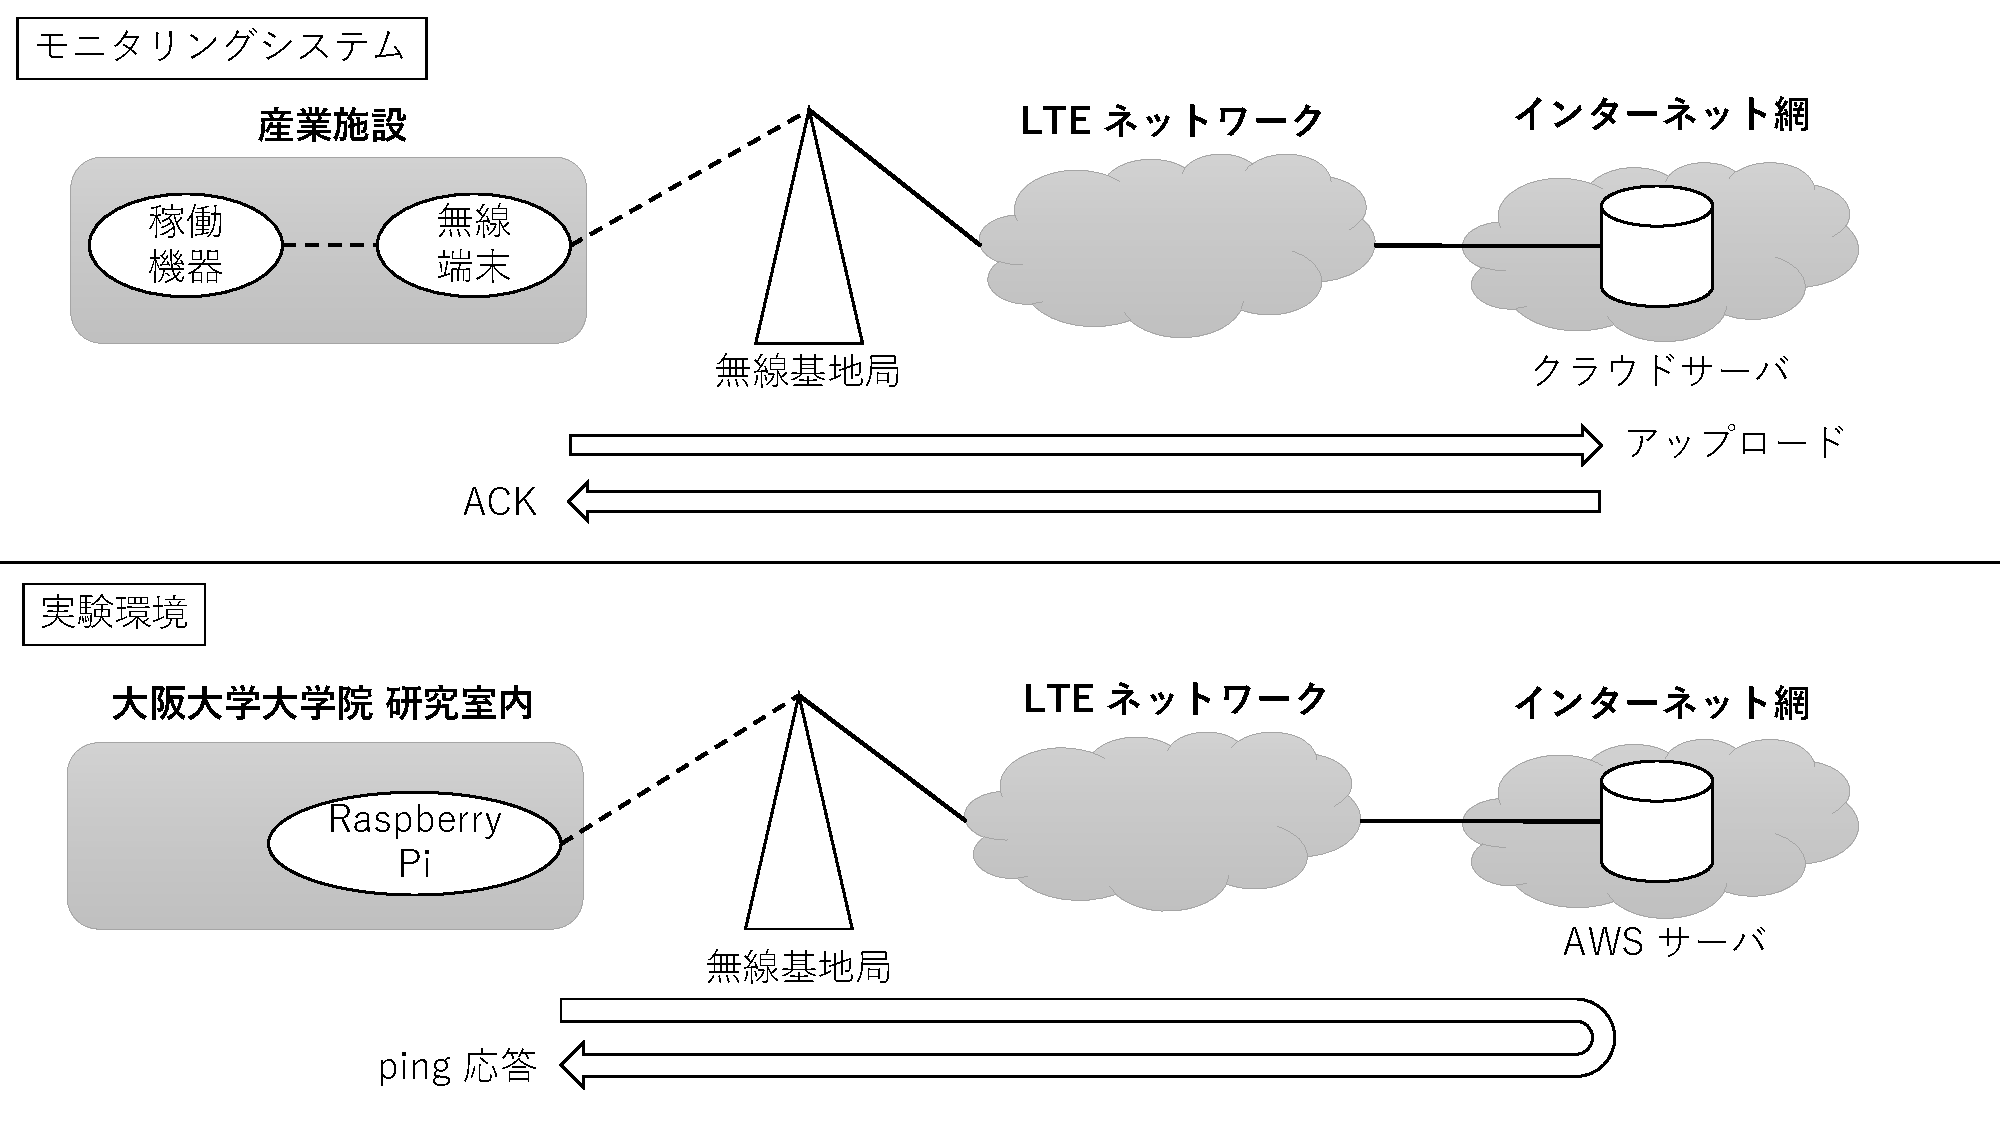
\includegraphics[width=10.0cm]{../figure/experiment.pdf}
\caption{モニタリングシステムと実験設定の対応}
\label{exp}
\end{figure}

\begin{table}[H]
\centering
\caption{実験の計測日時,対象}
\label{keisoku}
\begin{tabular}{|p{7cm}|p{7cm}|}
\hline
計測日時&対象\\
\hline
2/22(土)から 2/28(金)までのそれぞれ 3:00-4:00,7:00-8:00,12:00-13:00,17:00-18:00,20:00-21:00& AWS のウェブサーバ(aws.amazon.com)\\
\hline
2/22(土)から 3/18(水)までのそれぞれ 3:00-4:00,7:00-8:00,12:00-13:00,17:00-18:00,20:00-21:00& yahoo ニュースのサーバ(news.yahoo.co.jp)\\
\hline
2/29(土)から 3/18(水)までのそれぞれ 3:00-4:00,7:00-8:00,12:00-13:00,17:00-18:00,20:00-21:00&  AWS サーバ(13.114.202.235)\\
\hline
\end{tabular}
\end{table}

\section{計測結果}
 2/29(土)に行った AWS サーバを対象とした計測実験における ping 応答遅延を図 \ref{data} に示す.
ping 応答遅延の計測データを縦軸に取り,横軸に計測開始時のものから 1 から順に割り振ったインデックス $t$ を取った.
縦軸の範囲は 0ms から 400ms までとし,100ms から 400ms までの区間は縮小してある.
また,各図の上にそのデータの平均と分散を記した.

\begin{figure}[H]
\begin{center}
\subfigure[3:00 - 4:00]{
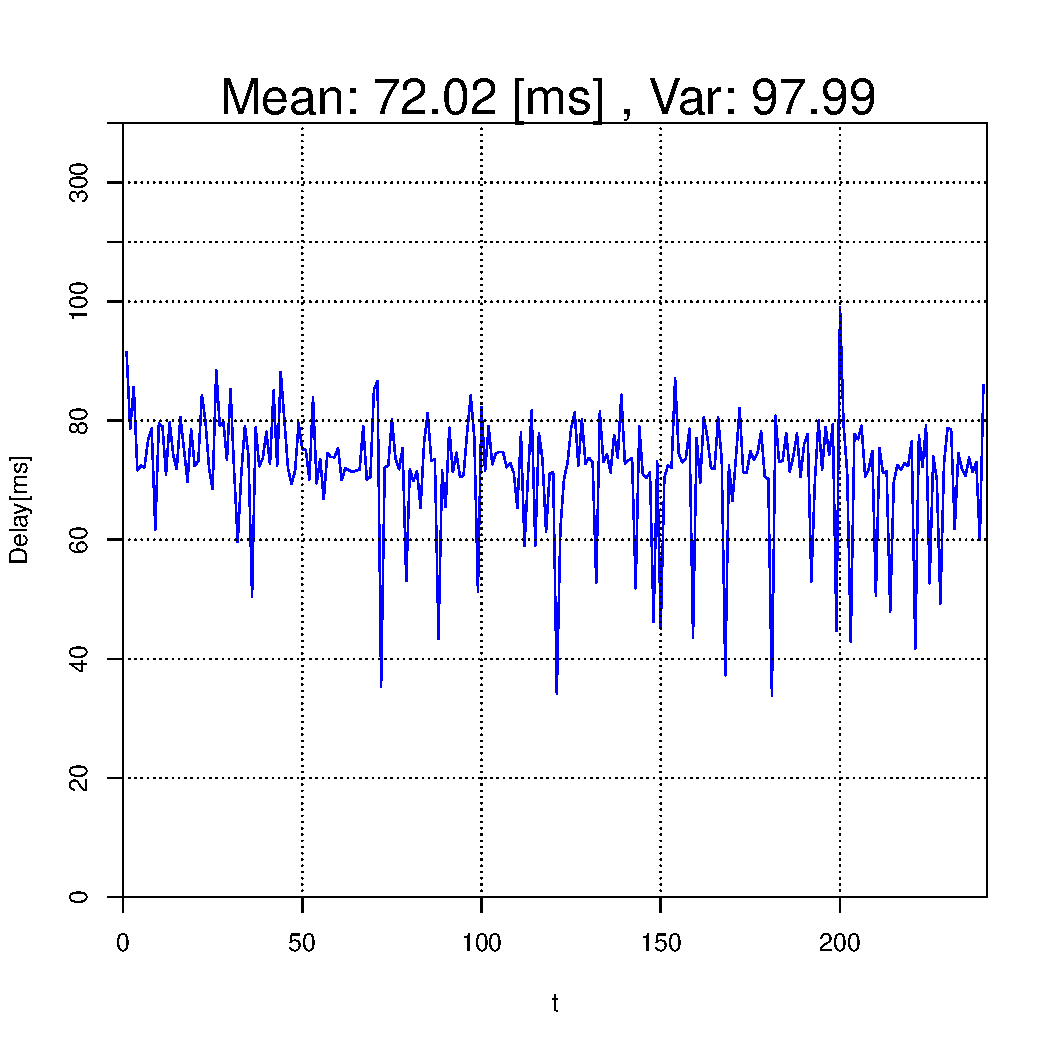
\includegraphics[width=.33\columnwidth]{C:/master/mstudy/analysis/plot/AWS/20200229_030001-plot.pdf}
}~
\subfigure[7:00 - 8:00]{
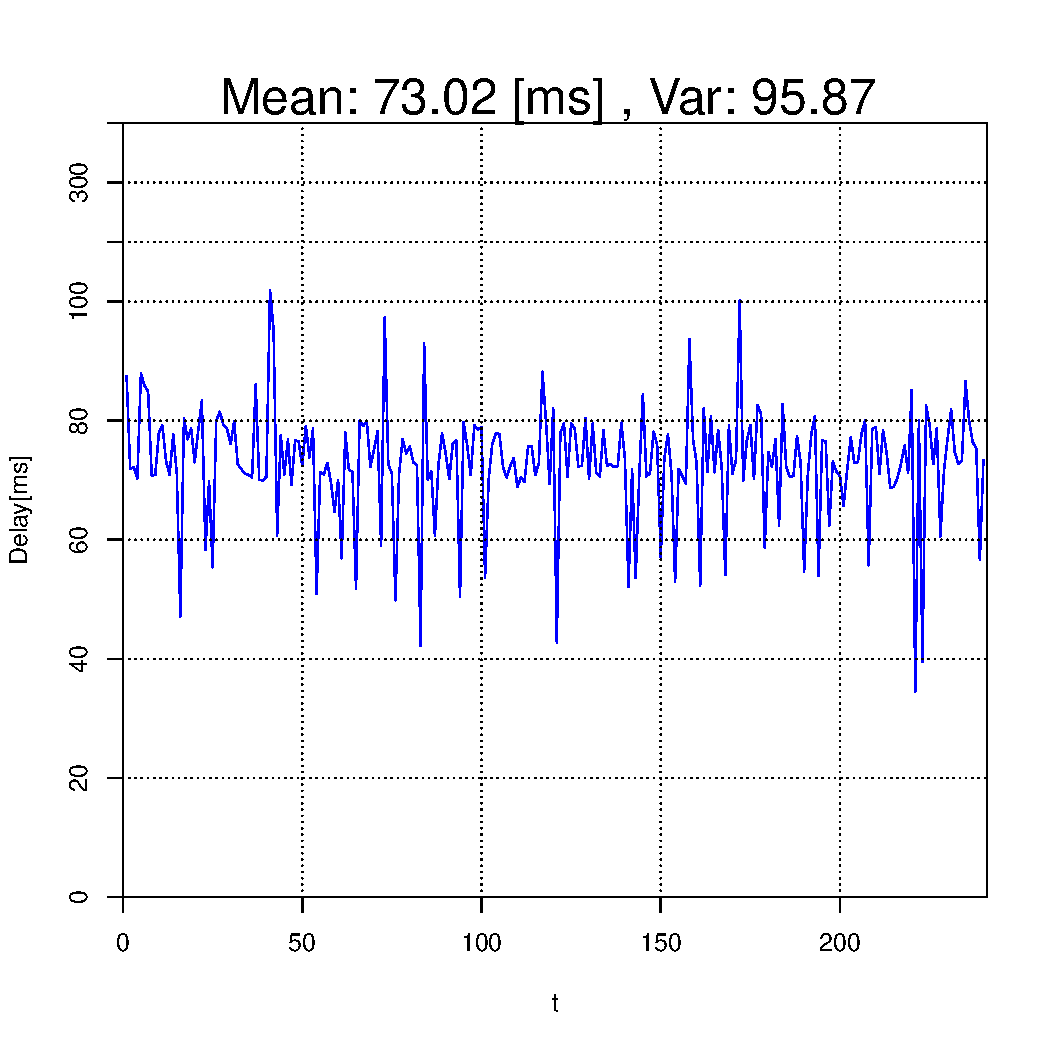
\includegraphics[width=.33\columnwidth]{C:/master/mstudy/analysis/plot/AWS/20200229_070001-plot.pdf}
}~
\subfigure[12:00 - 13:00]{
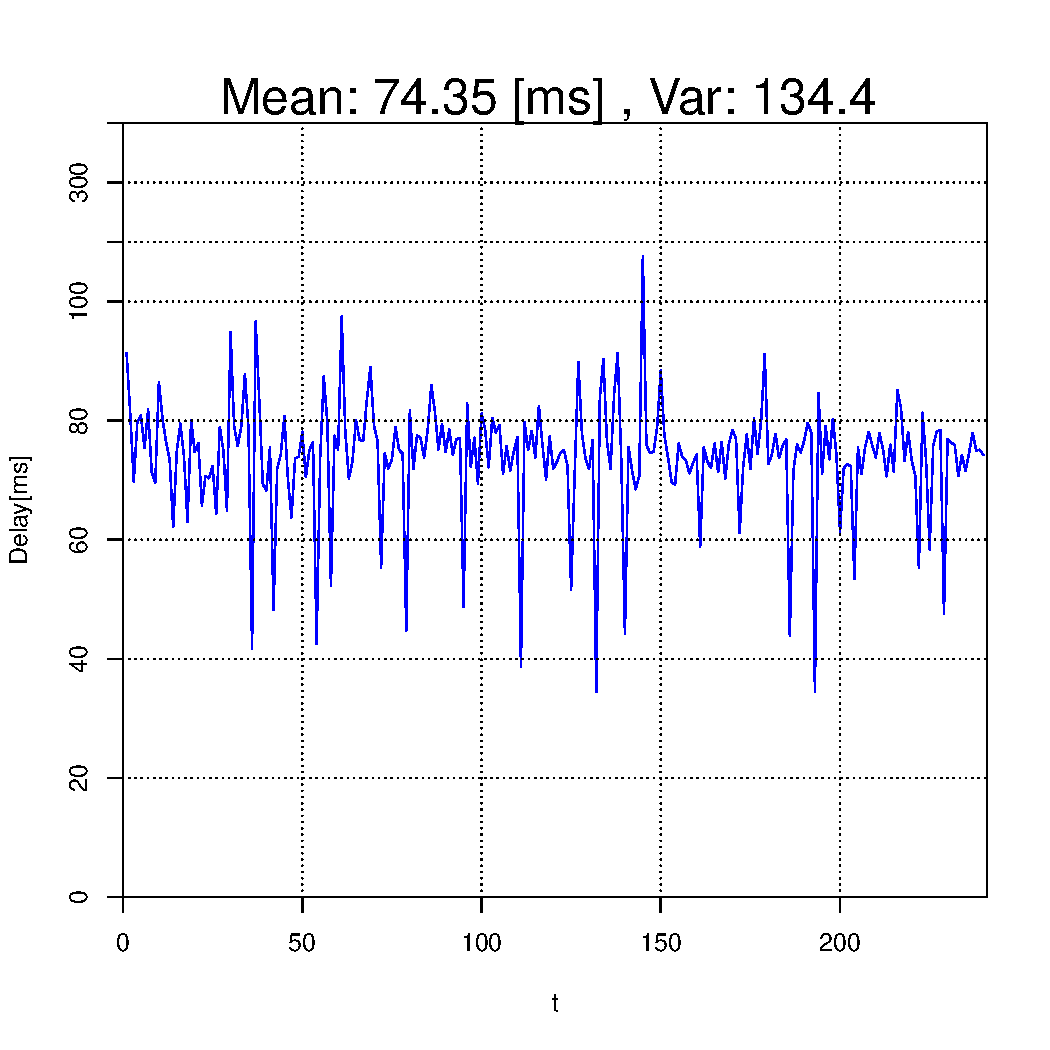
\includegraphics[width=.33\columnwidth]{C:/master/mstudy/analysis/plot/AWS/20200229_120001-plot.pdf}
}\\
\subfigure[17:00 - 18:00]{
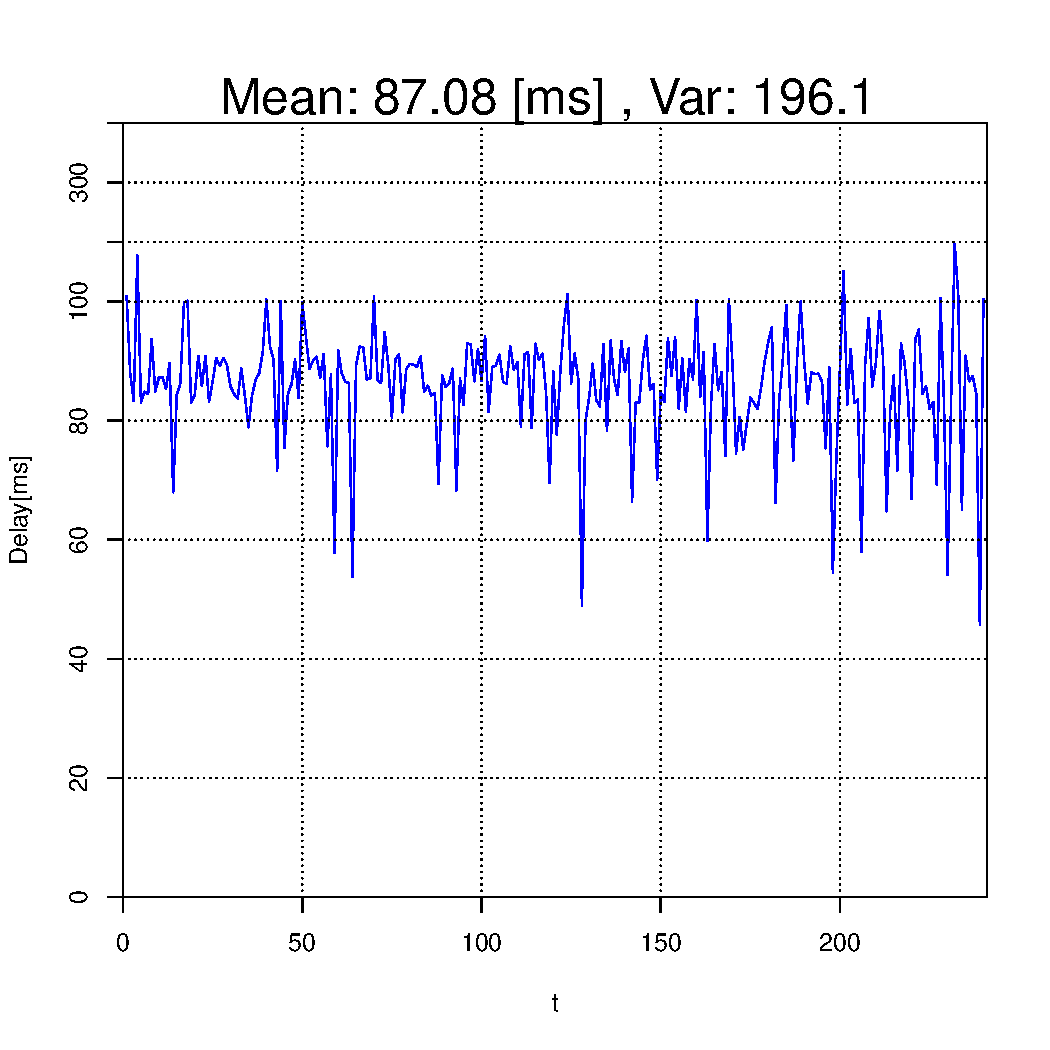
\includegraphics[width=.33\columnwidth]{C:/master/mstudy/analysis/plot/AWS/20200229_170002-plot.pdf}
}~
\subfigure[20:00 - 21:00]{
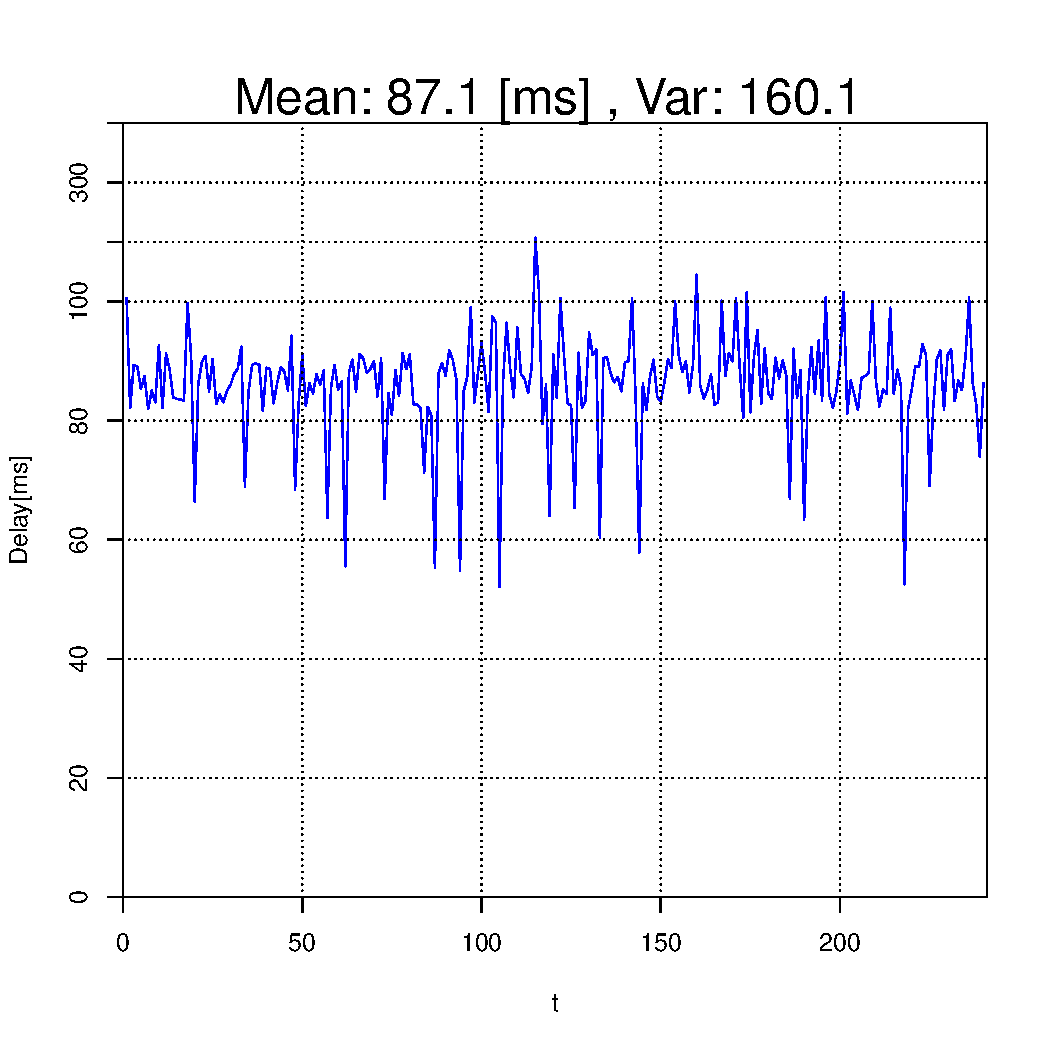
\includegraphics[width=.33\columnwidth]{C:/master/mstudy/analysis/plot/AWS/20200229_200001-plot.pdf}
}
\caption{2月29日(土) AWS サーバを対象とした ping 応答遅延}
\label{data}
\end{center}
\end{figure}
 
AWS サーバを対象とした計測データの平均値は,70ms 前半のものと 80ms 後半のものが見て取れる.
また,特徴として単発的に 40ms 程度の小さな応答遅延が発生するようだ.
traceroute による経路は,主に二つ確認できた.
\begin{table}[H]
\begin{tabular}{l}
 1  *\\
 2  *\\
 3  osk004ix51.IIJ.Net(58.138.106.30),osk004ix51.IIJ.Net(58.138.106.130),...\\
 4  210.173.178.59(210.173.178.59),210.173.178.59(210.173.178.61)\\
 5  *\\
 6  *\\
 7  *\\
 8  54.239.53.10(54.239.53.10),54.239.53.12(54.239.53.12),...\\
 9  *\\
10  *\\
11  52.95.31.159(52.95.31.159),52.95.31.161(52.95.31.161),...\\
12  *\\
13  *\\
14  52.95.30.208(52.95.30.208),52.95.30.212(52.95.30.212),...\\
15  *\\
16  *\\
============\\
120 *\\
\end{tabular}
\end{table}

また,

\begin{table}[H]
\begin{tabular}{l}
 1  *\\
 2  tky008nasgw110.IIJ.Net(160.13.52.241),tky008nasgw110.IIJ.Net (160.13.52.245),...\\
 3  *\\
 4  tky001bb10.IIJ.Net(58.138.80.97),tky001bb10.IIJ.Net(58.138.88.1),...\\
 5  tky001ix11.IIJ.Net(58.138.102.202),tky001ix11.IIJ.Net(58.138.102.202),...\\
 6  210.173.176.188(210.173.176.188),210.173.176.198(210.173.176.198)\\
 7  *\\
 8  *\\
 9  *\\
10  52.95.30.10(52.95.30.10),52.95.30.12(52.95.30.12),...\\
11  *\\
12  *\\
13  *\\
14  *\\
15  52.95.31.159(52.95.31.159),52.95.31.161(52.95.31.161),...\\
16  *\\
17  *\\
18  52.95.30.208(52.95.30.208),52.95.30.212(52.95.30.212),...\\
19  *\\
=============\\
120  *\\
\end{tabular}
\end{table}
となっていた.

上段の 4 ホップ目は大阪にある IX であり,下段の 6 ホップ目は東京にある IX である.
また,これ以降に確認できる機器はすべて Amazon のネットワーク内の機器であり所在地は日本であった.
しかし,計測対象の AWS サーバから 120 ホップ以内で traceroute 応答を得ることはできなかった.
\section{ARMA モデルによる回帰}
\subsection{データの前処理}
\subsubsection{定常性の確認}
多くの時系列モデルでは,対象データに定常性を仮定しており,ARMA モデルもそのひとつである.
そのため,ARMA モデルを適用するにあたり,まず AWS サーバを計測対象とした ping 応答遅延データが定常性を満たすか確認する必要がある.
その手段として,非定常であることを帰無仮説,定常であることを対立仮説とした単位根検定が知られている.
ここでは,その一つの拡張ディッキー–フラー検定(ADF検定)を用い,AWS サーバからの ping 応答遅延データが定常性を満たすかを確認した結果,12/29(土)に計測した五つのデータにおいて,それぞれの p 値はすべて 0.01 以下となった.
よって,非定常であるという帰無仮説は棄却され定常性を満たすことが確認できた.

\subsubsection{データの前処理}
データの前処理として次を検討する.\\
(i)前処理なし\\
(ii)差分処理を行う\\
(iii)指数移動平均($移動平均系列_t = 0.1*計測データ_t + 0.9*移動平均系列_{t-1}$)
\subsubsection{ARMA モデル}
回帰対象のデータ系列を $\{y_t\}^N_{t=1}$ として,ARMA モデルは次式で与えられる.
$$\displaystyle y_t = c + \sum^p_{i=1}a_iy_i + \sum^q_{j=1}b_j\varepsilon_j + \varepsilon_t \hspace{0.5cm} \varepsilon_t \sim N(0,\sigma^2) \verb|i.i.d|$$

モデルのパラメータ数を表す次数$ (p,q) $は AIC を基に最大値で統一する.
(i)(ii)は $0 \le p \le 2 , 0 \le q \le 2$,(iii) は $0 \le p \le 1 , 0 \le q \le 1$を探索範囲とした.
結果は,(i)(ii)は $(p,q)=(2,2)$ ,(iii)は $(p,q)=(1,1)$ となった.

(i)(ii)(iii)それぞれの回帰結果のうち,12/29(土)のものを図 \ref{reg1} から図\ref{reg2} に示す.
\begin{figure}[H]
\begin{center}
\subfigure[3:00 - 4:00]{
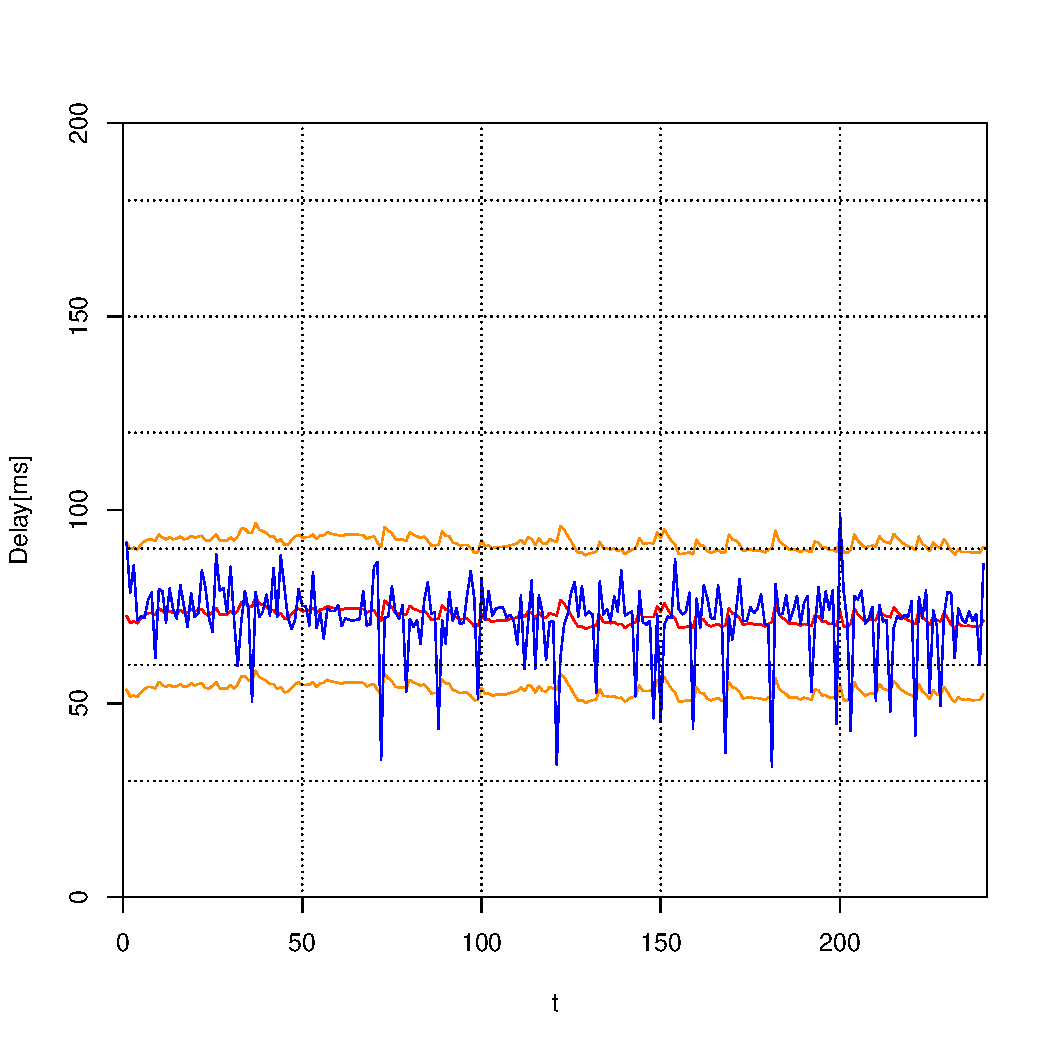
\includegraphics[width=.33\columnwidth]{C:/master/mstudy/paper/figure/0229_03-arma-normal.pdf}
}~
\subfigure[7:00 - 8:00]{
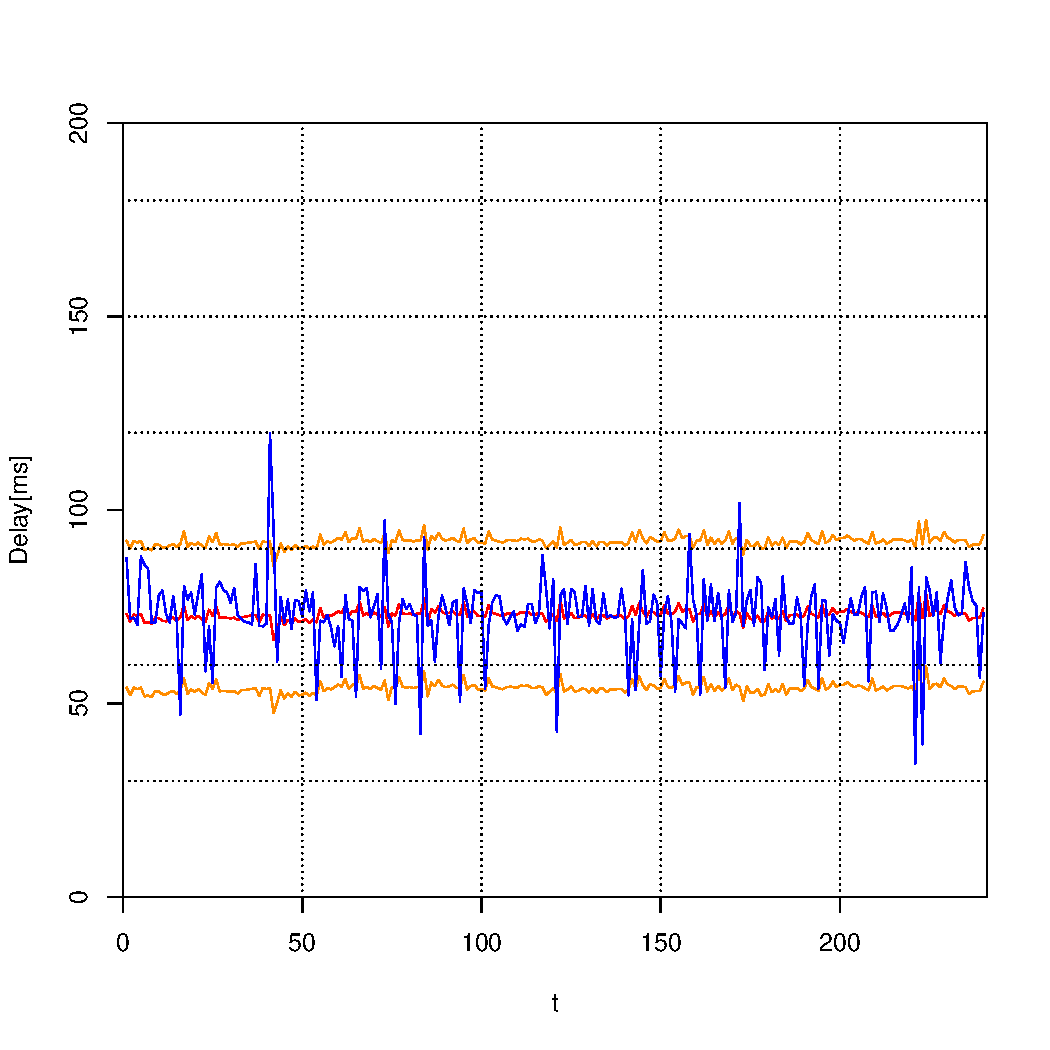
\includegraphics[width=.33\columnwidth]{C:/master/mstudy/paper/figure/0229_07-arma-normal.pdf}
}~
\subfigure[12:00 - 13:00]{
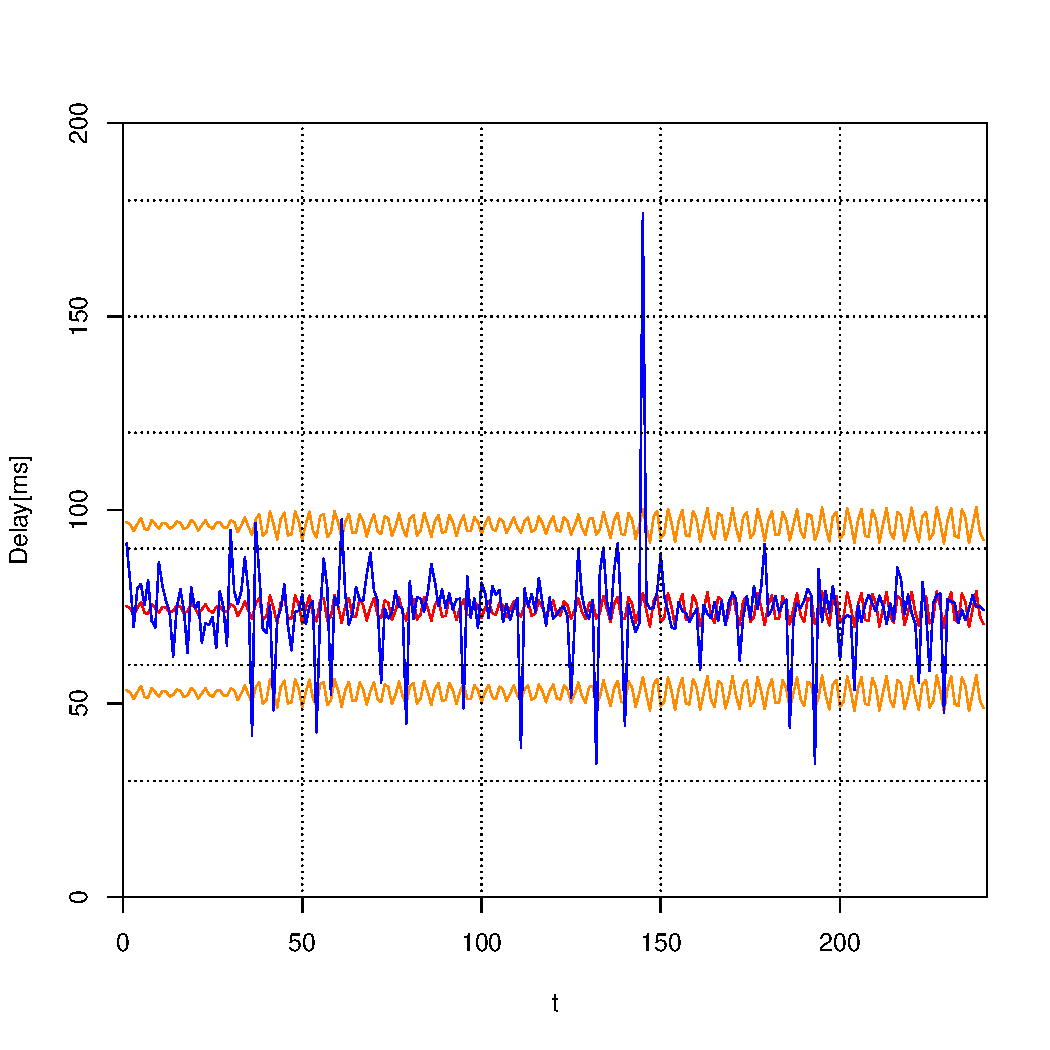
\includegraphics[width=.33\columnwidth]{C:/master/mstudy/paper/figure/0229_12-arma-normal.pdf}
}\\
\subfigure[17:00 - 18:00]{
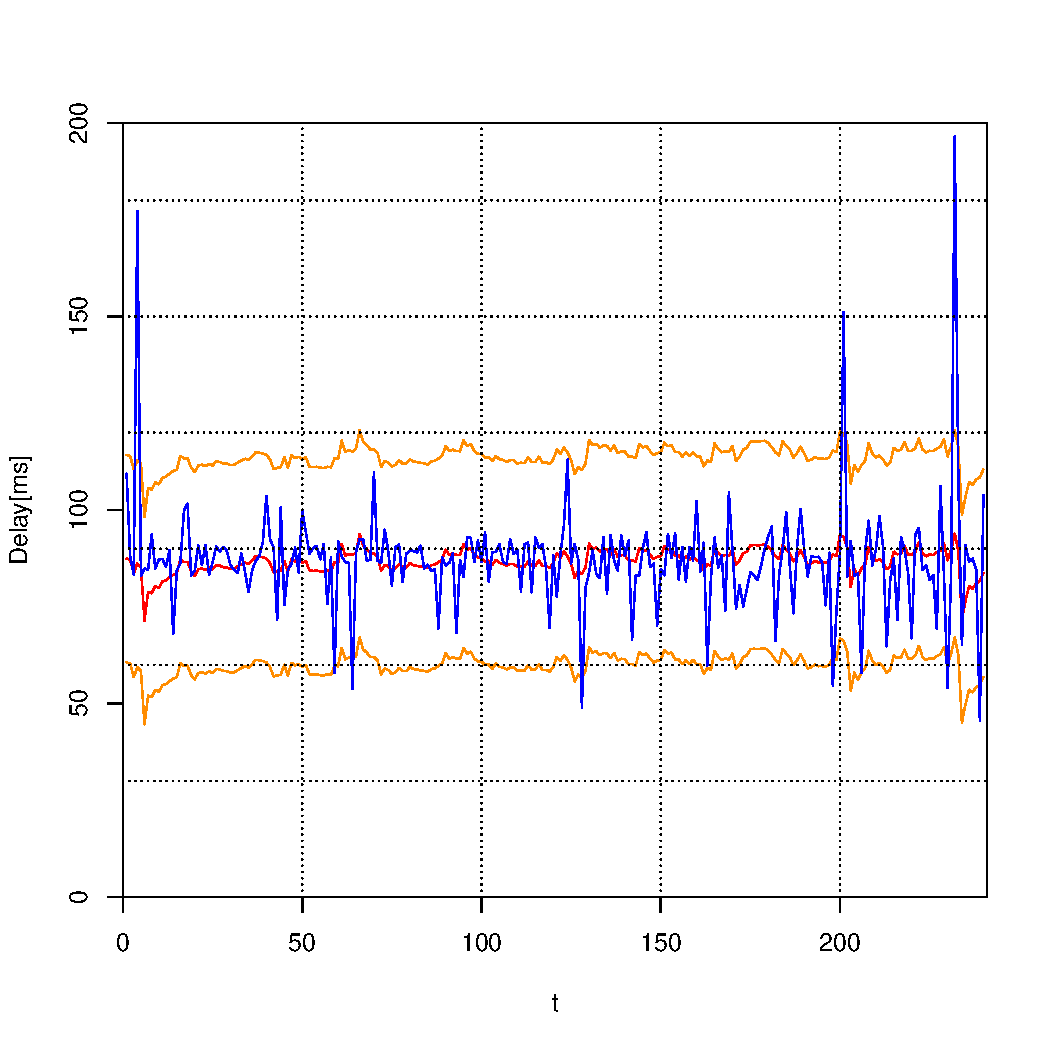
\includegraphics[width=.33\columnwidth]{C:/master/mstudy/paper/figure/0229_17-arma-normal.pdf}
}~
\subfigure[20:00 - 21:00]{
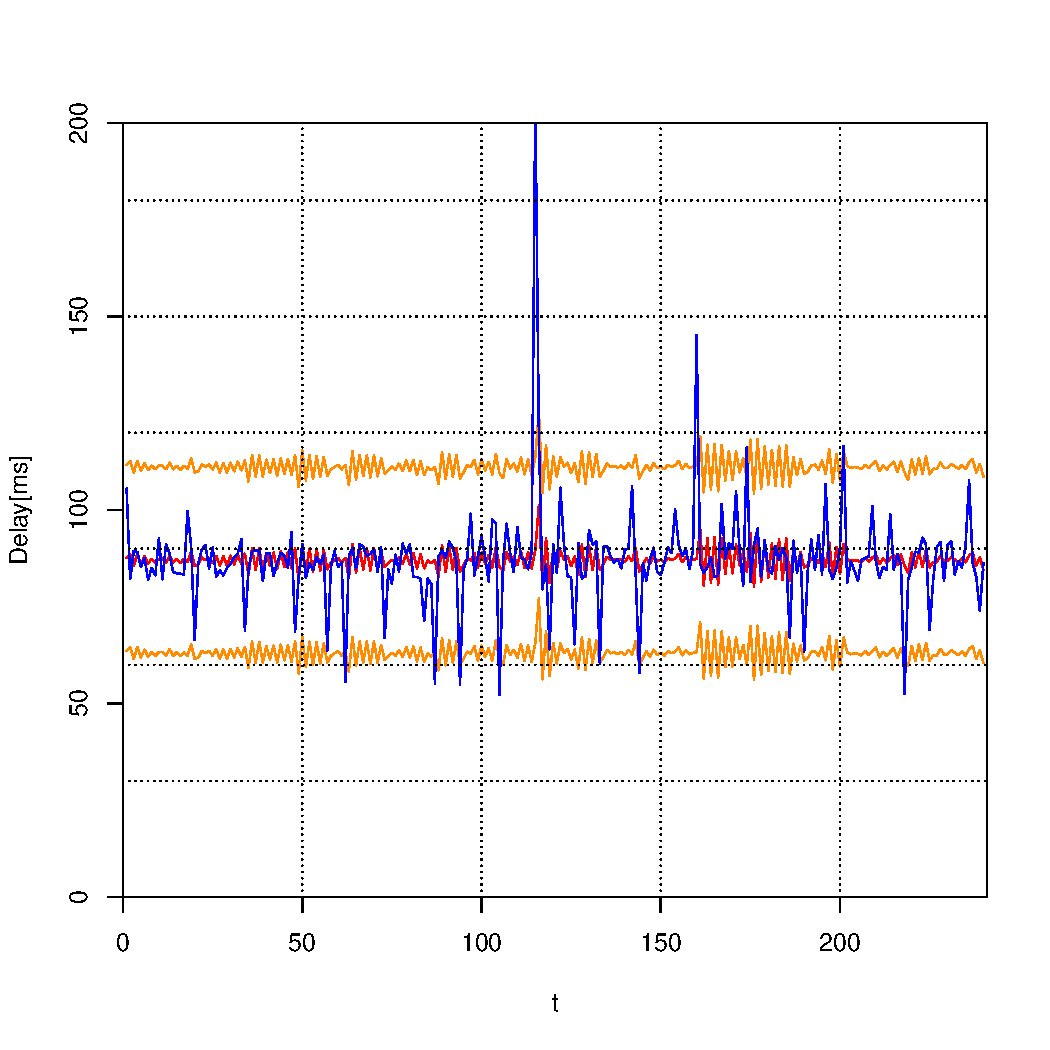
\includegraphics[width=.33\columnwidth]{C:/master/mstudy/paper/figure/0229_20-arma-normal.pdf}
}
\caption{2月29日(土) AWS サーバを対象とした ping 応答遅延に対する(i)前処理なしでの ARMA モデル回帰(青線:実測値,赤線:推定値,橙線範囲:信頼区間 95\% )}
\label{reg1}
\end{center}
\end{figure}

\begin{figure}[H]
\begin{center}
\subfigure[3:00 - 4:00]{
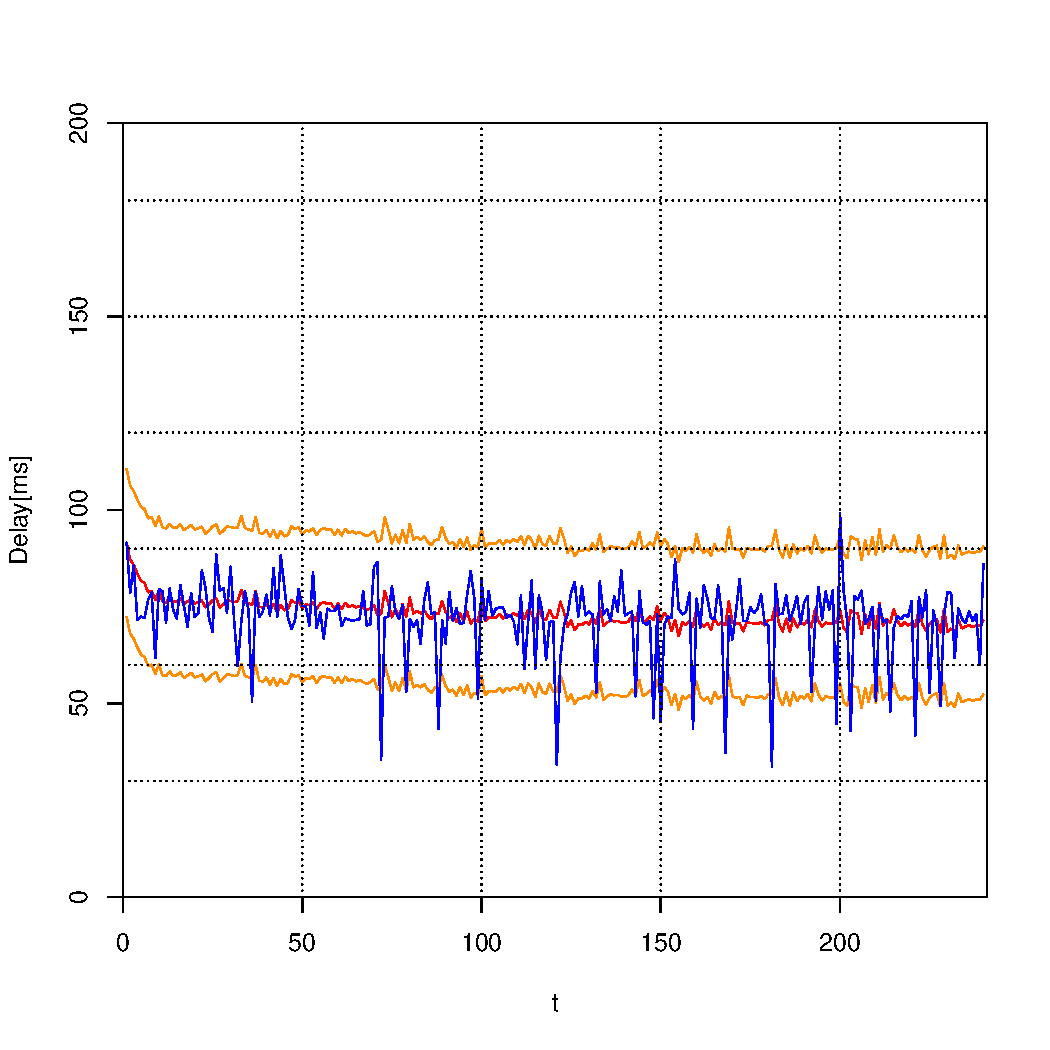
\includegraphics[width=.33\columnwidth]{C:/master/mstudy/paper/figure/0229_03-arma-diff.pdf}
}~
\subfigure[7:00 - 8:00]{
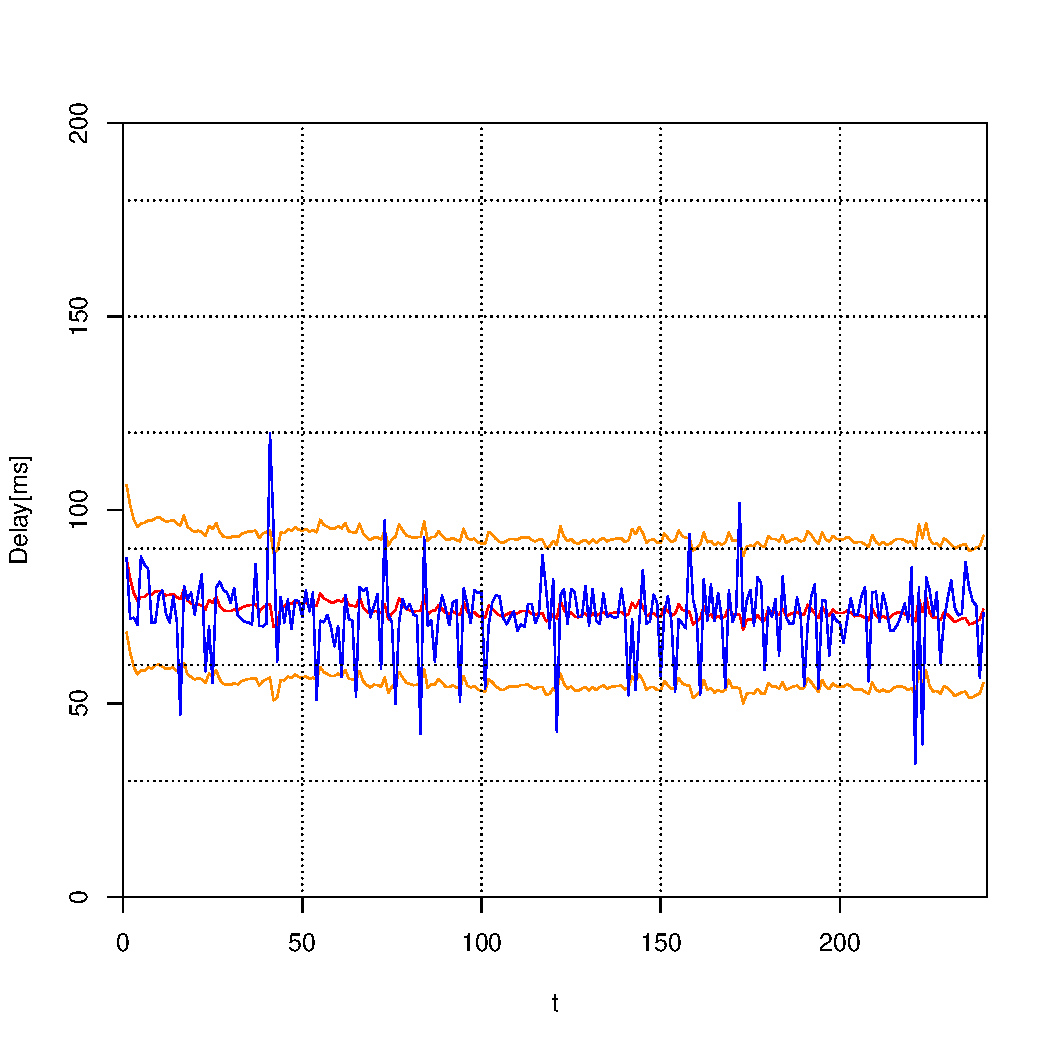
\includegraphics[width=.33\columnwidth]{C:/master/mstudy/paper/figure/0229_07-arma-diff.pdf}
}~
\subfigure[12:00 - 13:00]{
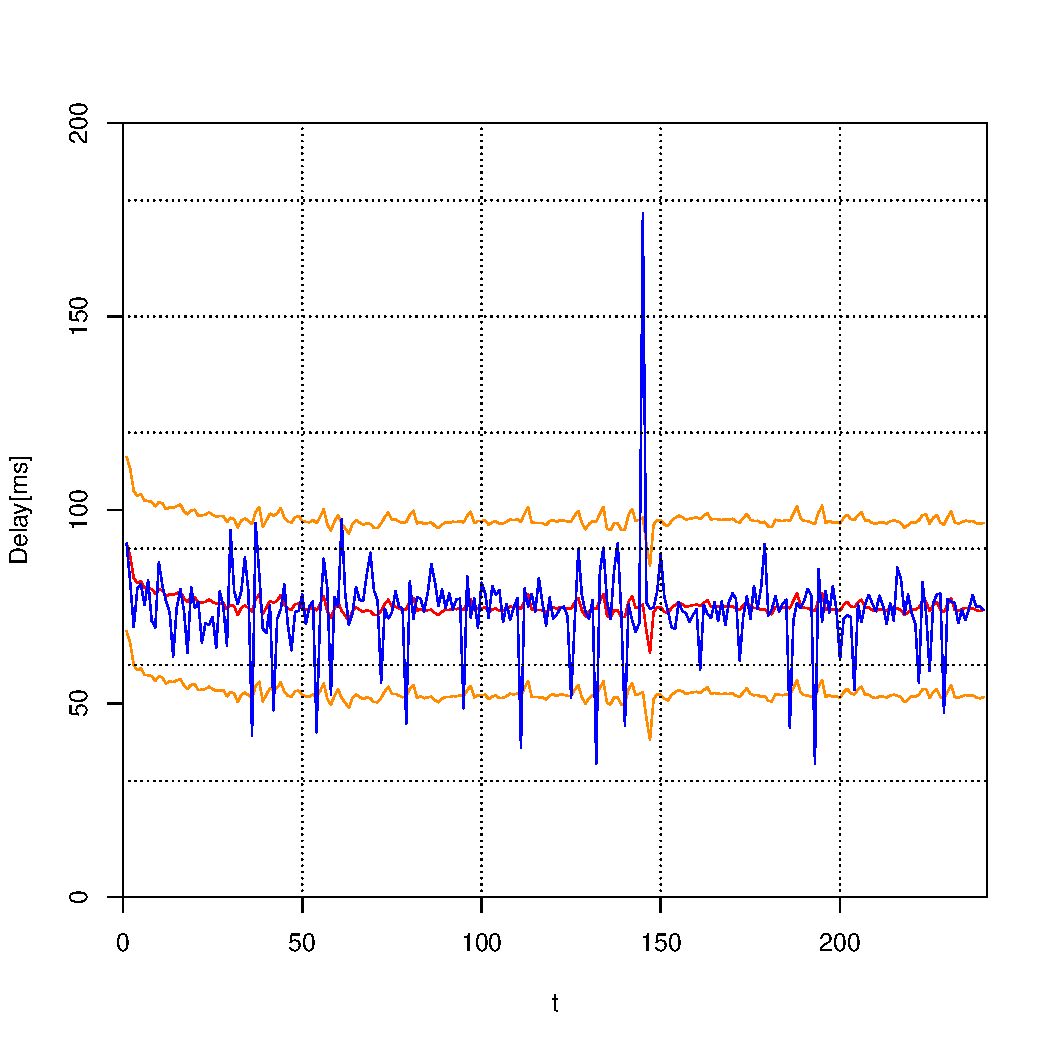
\includegraphics[width=.33\columnwidth]{C:/master/mstudy/paper/figure/0229_12-arma-diff.pdf}
}\\
\subfigure[17:00 - 18:00]{
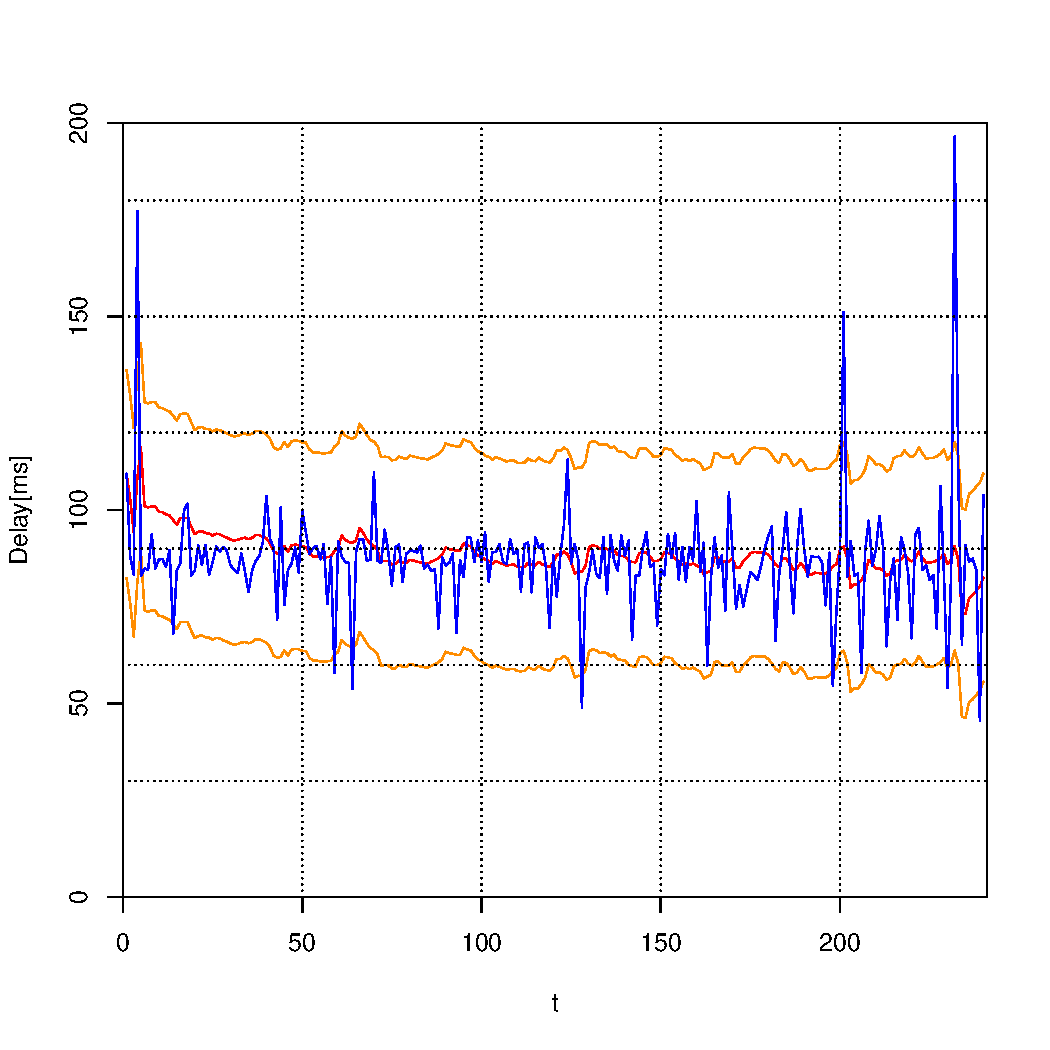
\includegraphics[width=.33\columnwidth]{C:/master/mstudy/paper/figure/0229_17-arma-diff.pdf}
}~
\subfigure[20:00 - 21:00]{
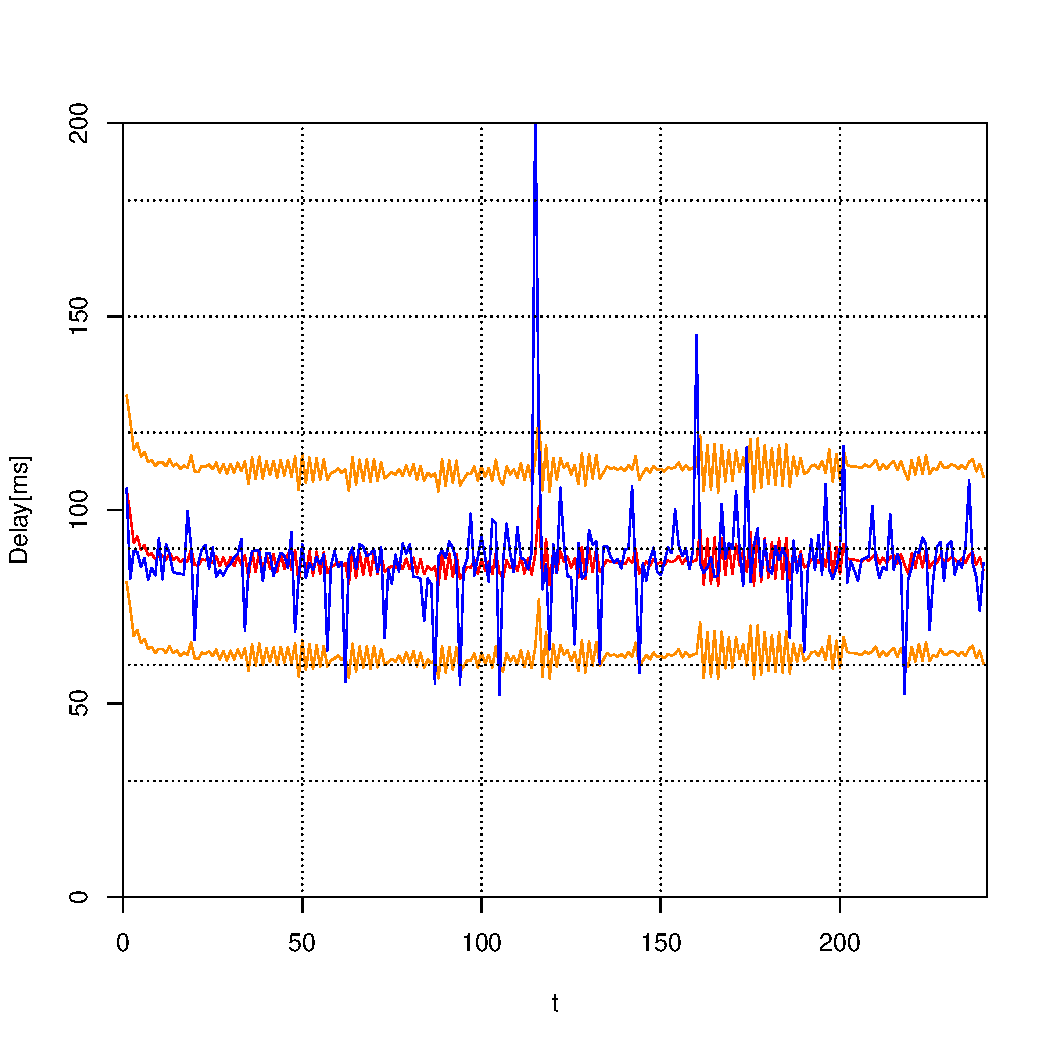
\includegraphics[width=.33\columnwidth]{C:/master/mstudy/paper/figure/0229_20-arma-diff.pdf}
}
\caption{2月29日(土) AWS サーバを対象とした ping 応答遅延に対する(ii)差分処理での ARMA モデル回帰(青線:実測値,赤線:推定値,橙線範囲:信頼区間 95\% )}
\end{center}
\end{figure}

\begin{figure}[H]
\begin{center}
\subfigure[3:00 - 4:00]{
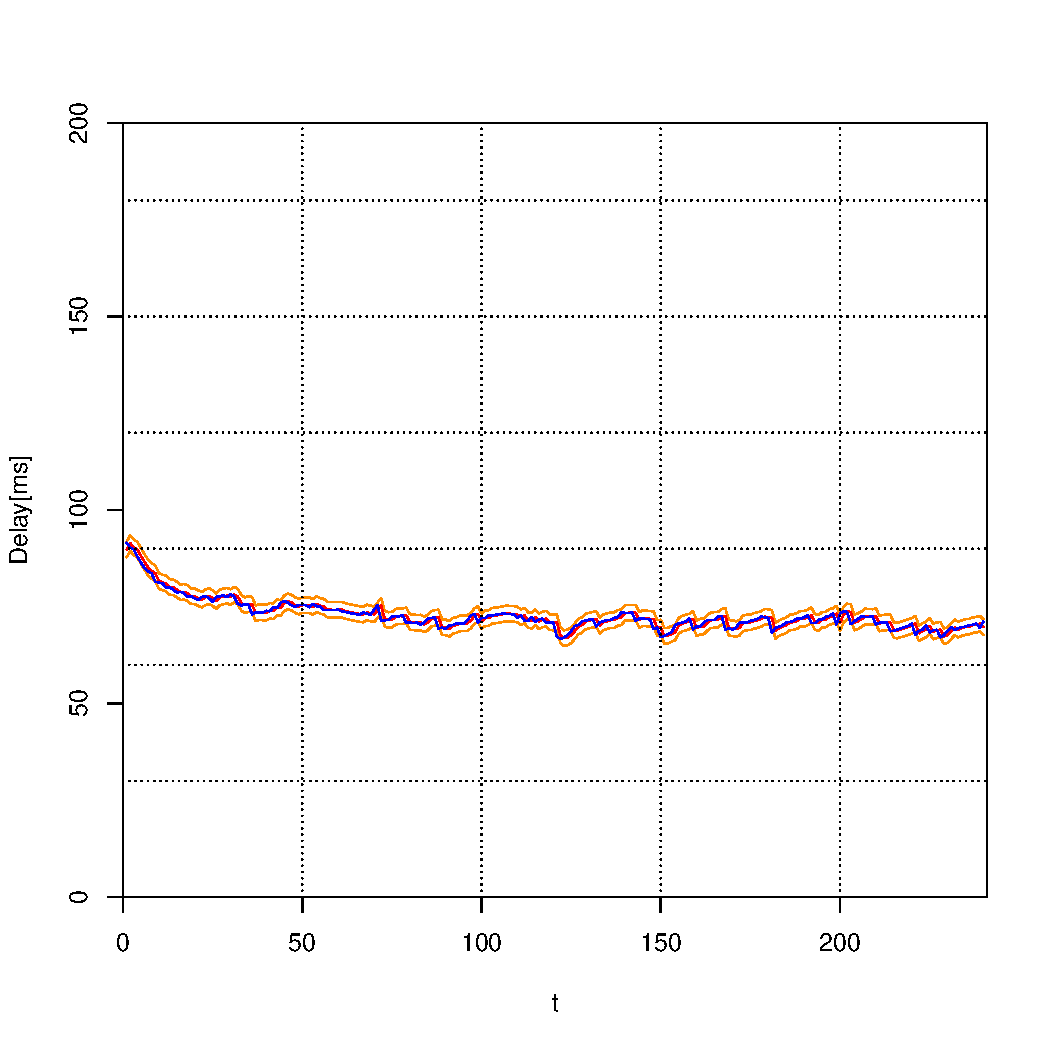
\includegraphics[width=.33\columnwidth]{C:/master/mstudy/paper/figure/0229_03-arma-ma.pdf}
}~
\subfigure[7:00 - 8:00]{
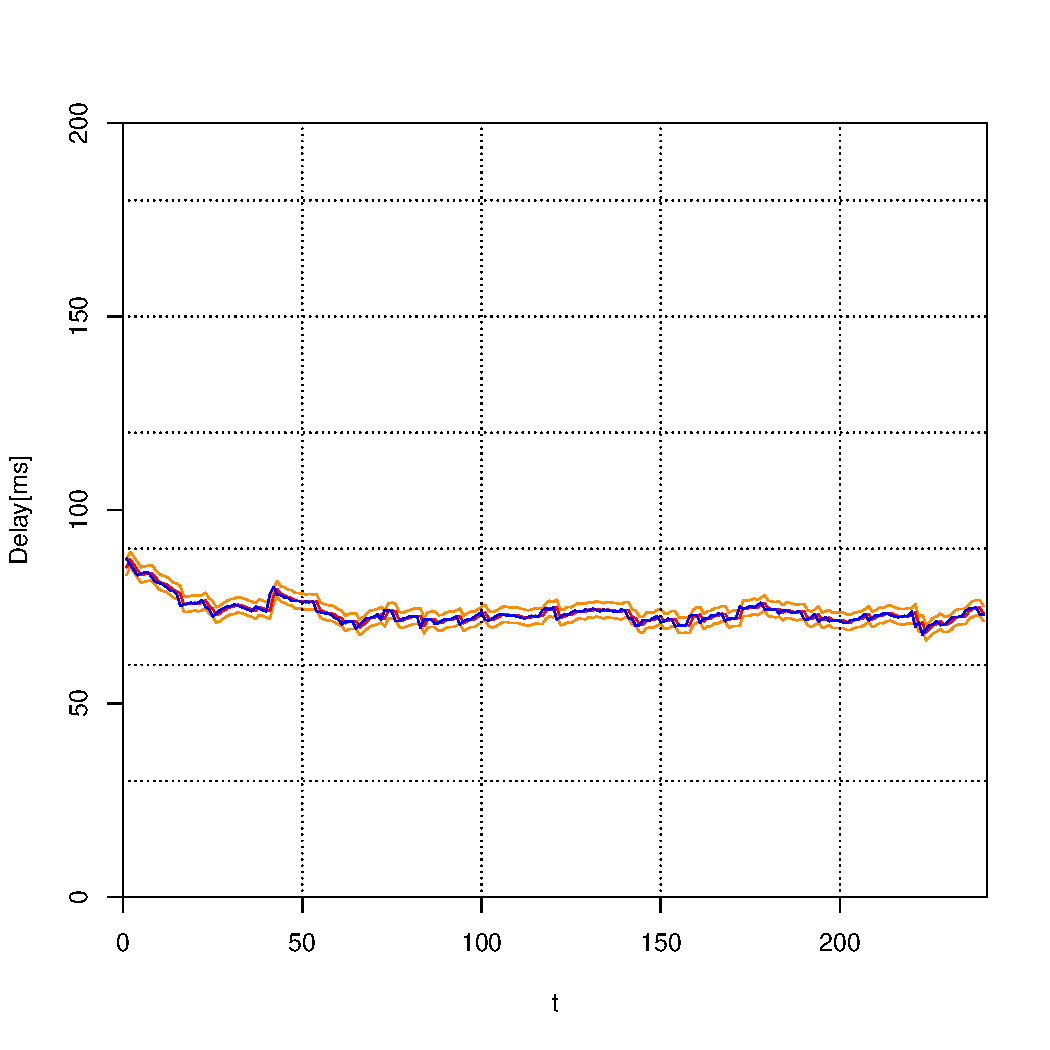
\includegraphics[width=.33\columnwidth]{C:/master/mstudy/paper/figure/0229_07-arma-ma.pdf}
}~
\subfigure[12:00 - 13:00]{
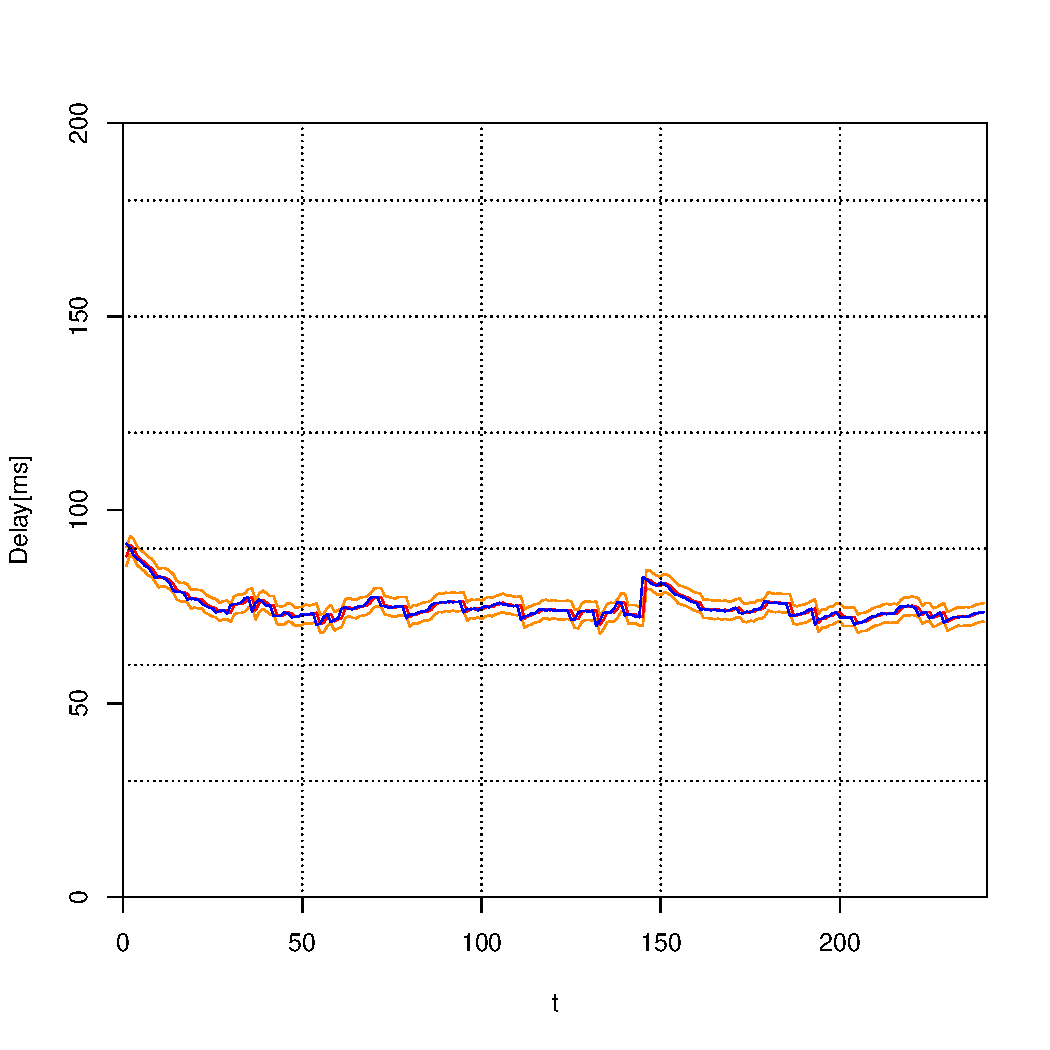
\includegraphics[width=.33\columnwidth]{C:/master/mstudy/paper/figure/0229_12-arma-ma.pdf}
}\\
\subfigure[17:00 - 18:00]{
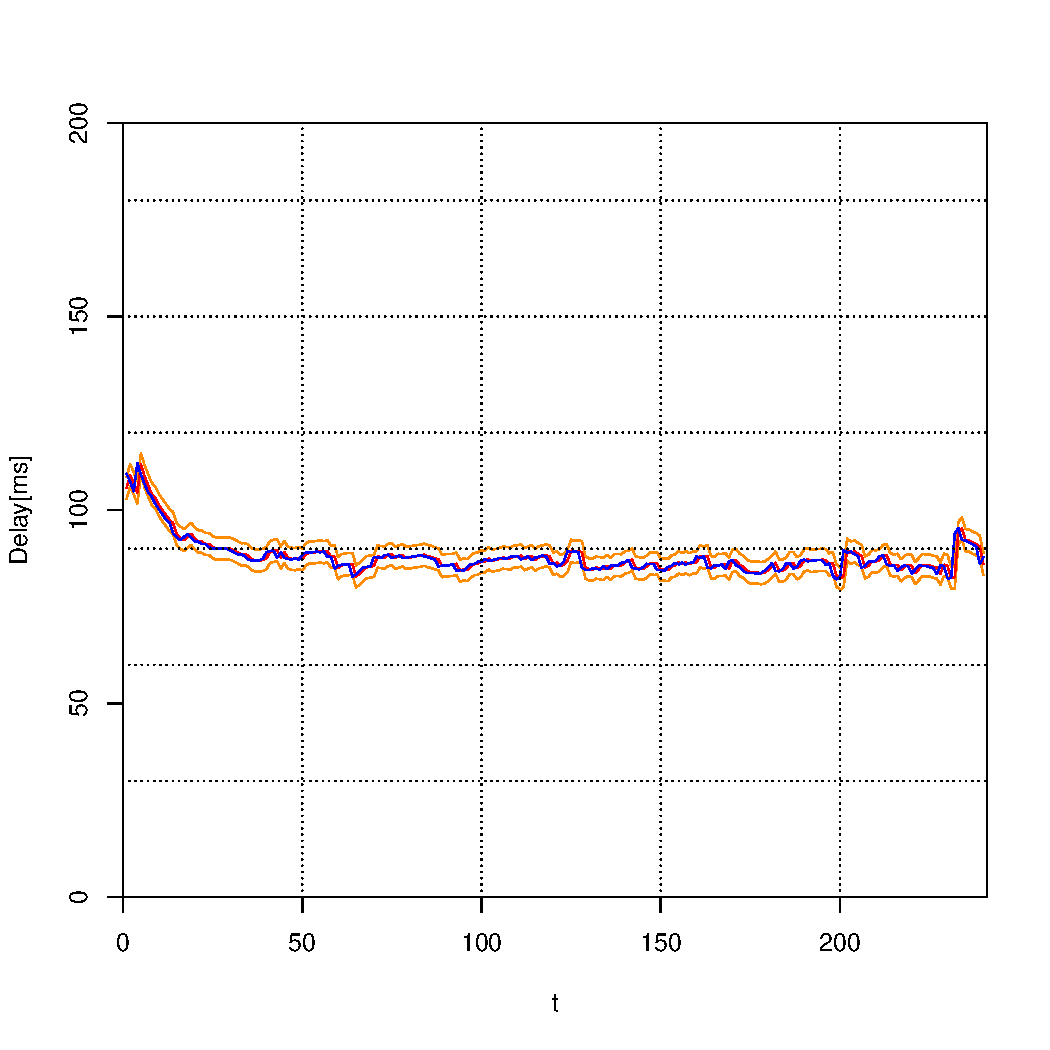
\includegraphics[width=.33\columnwidth]{C:/master/mstudy/paper/figure/0229_17-arma-ma.pdf}
}~
\subfigure[20:00 - 21:00]{
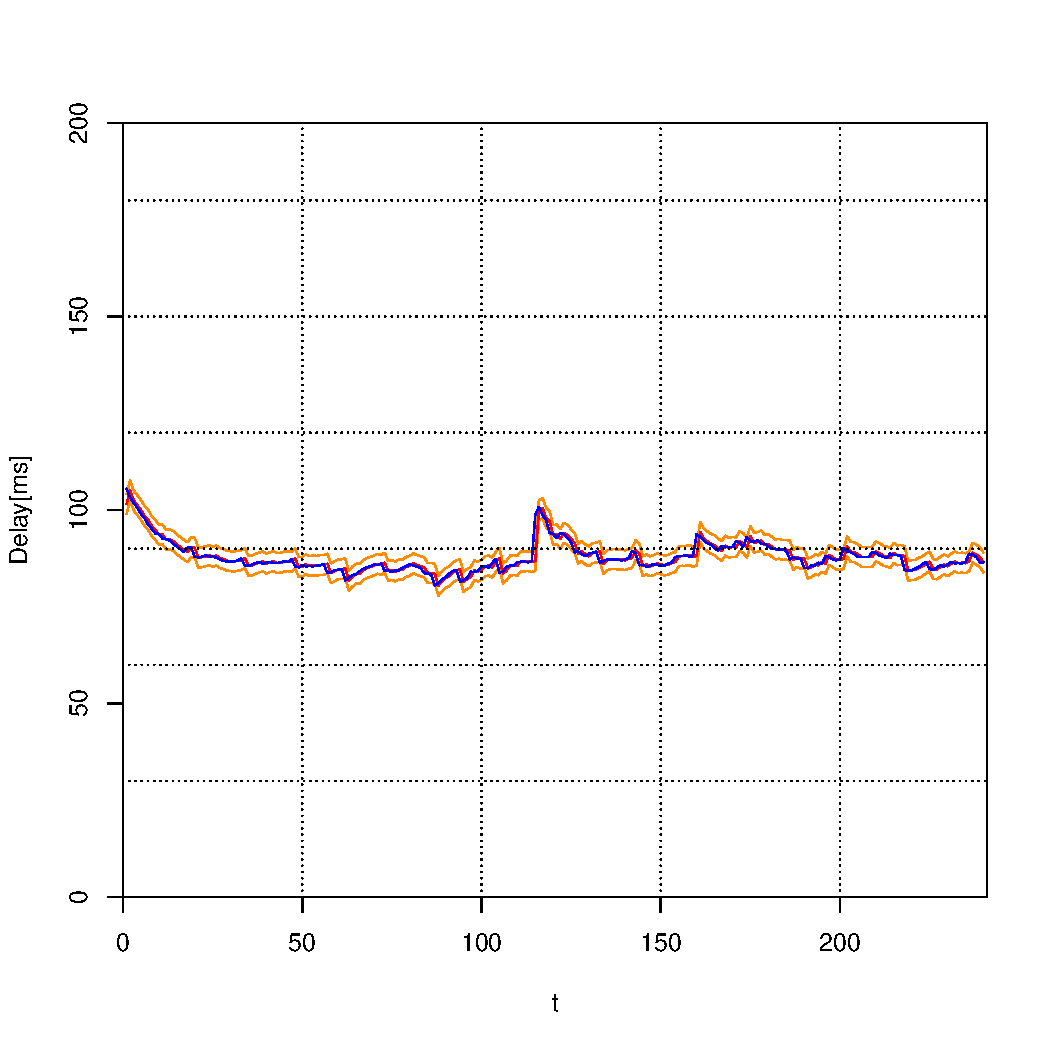
\includegraphics[width=.33\columnwidth]{C:/master/mstudy/paper/figure/0229_20-arma-ma.pdf}
}
\caption{2月29日(土) AWS サーバを対象とした ping 応答遅延に対する(iii)移動平均での ARMA モデル回帰(青線:移動平均系列,赤線:推定値,橙線範囲:信頼区間 95\% )}
\label{reg2}
\end{center}
\end{figure}

モデルの適切さを判断するためには,残差分析が必要である.
ARMA モデルの残差は平均 0 の正規分布に従い,それらは互いに独立であることが望ましい.
図 \ref{reg1} から図 \ref{reg2} のそれぞれの残差分布を図 \ref{res1} から図 \ref{res2} に示す.

\begin{figure}[H]
\begin{center}
\subfigure[3:00 - 4:00]{
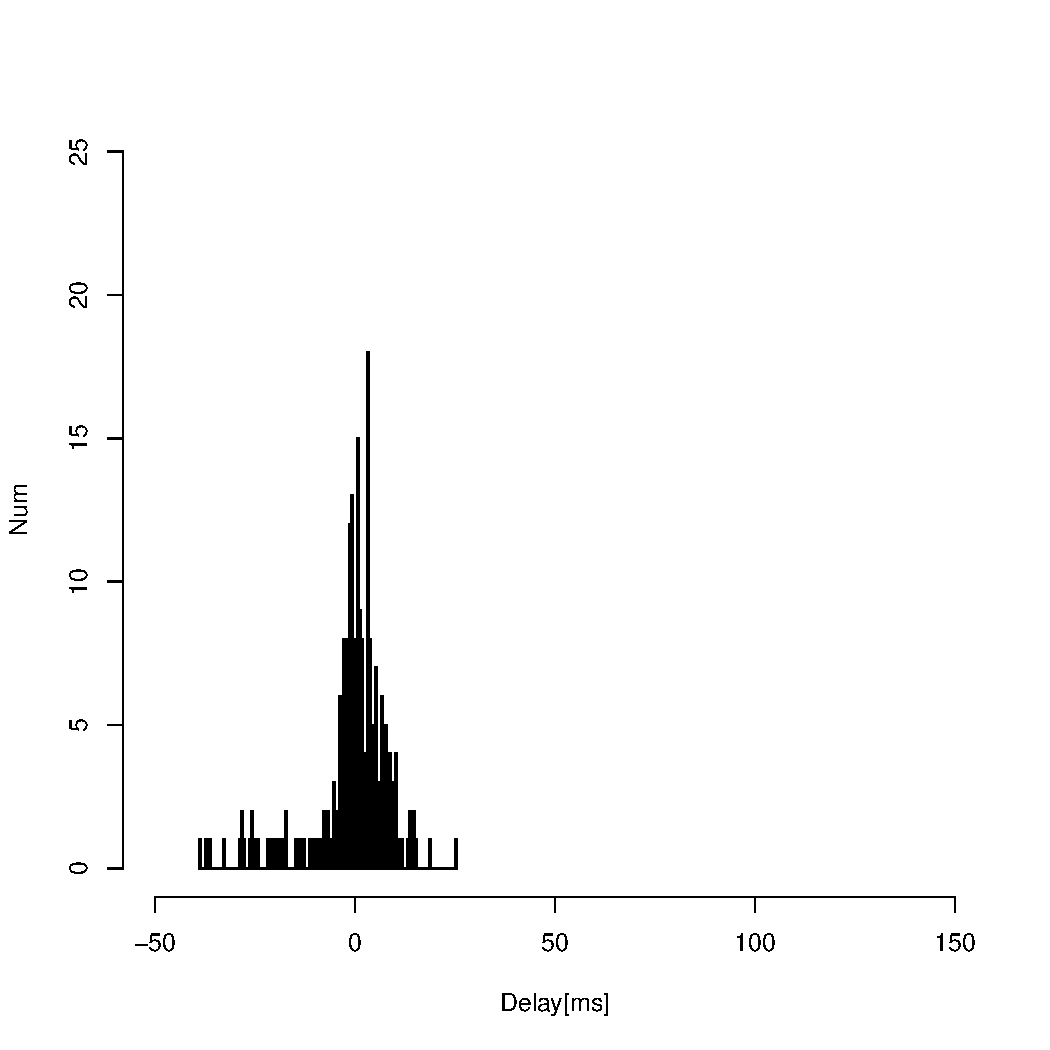
\includegraphics[width=.33\columnwidth]{C:/master/mstudy/paper/figure/0229_03-arma-normal-reshist.pdf}
}~
\subfigure[7:00 - 8:00]{
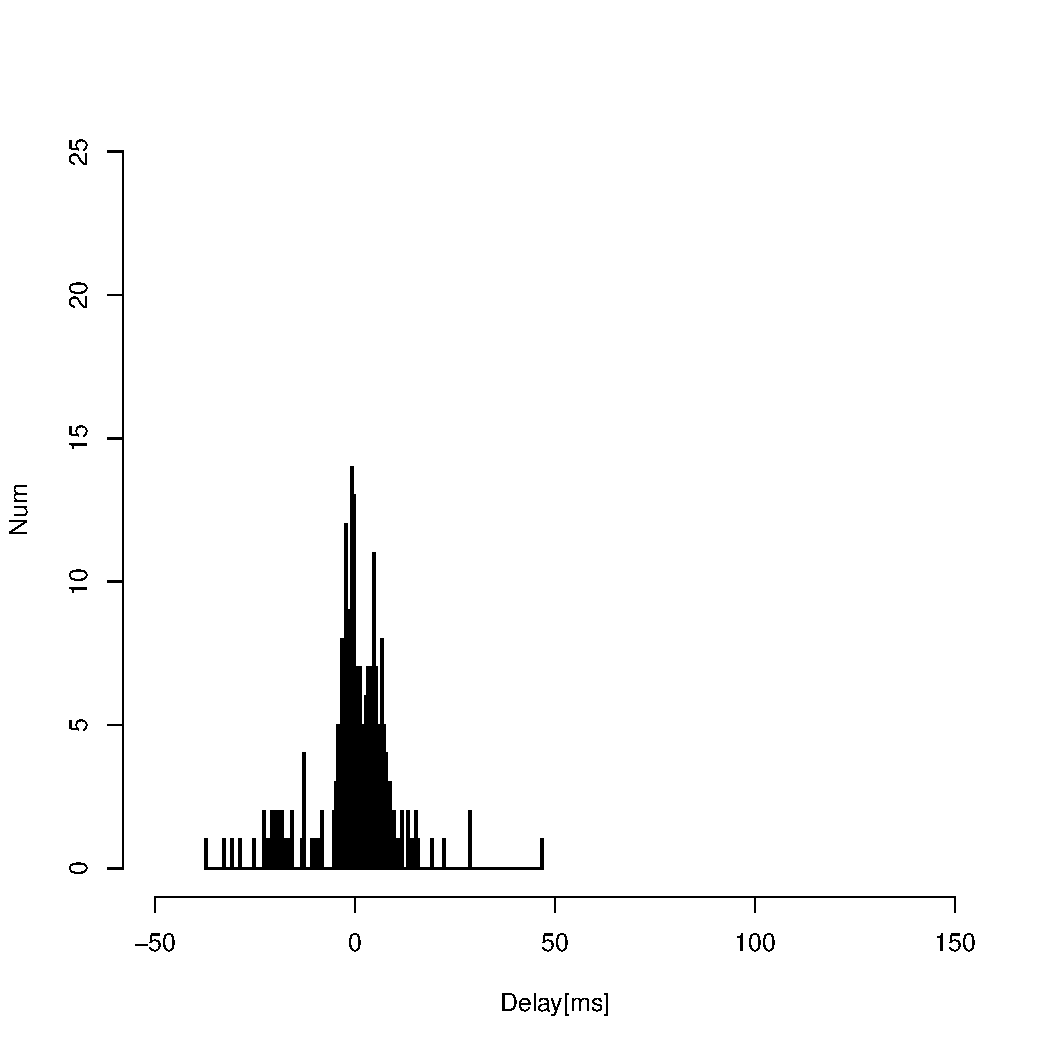
\includegraphics[width=.33\columnwidth]{C:/master/mstudy/paper/figure/0229_07-arma-normal-reshist.pdf}
}~
\subfigure[12:00 - 13:00]{
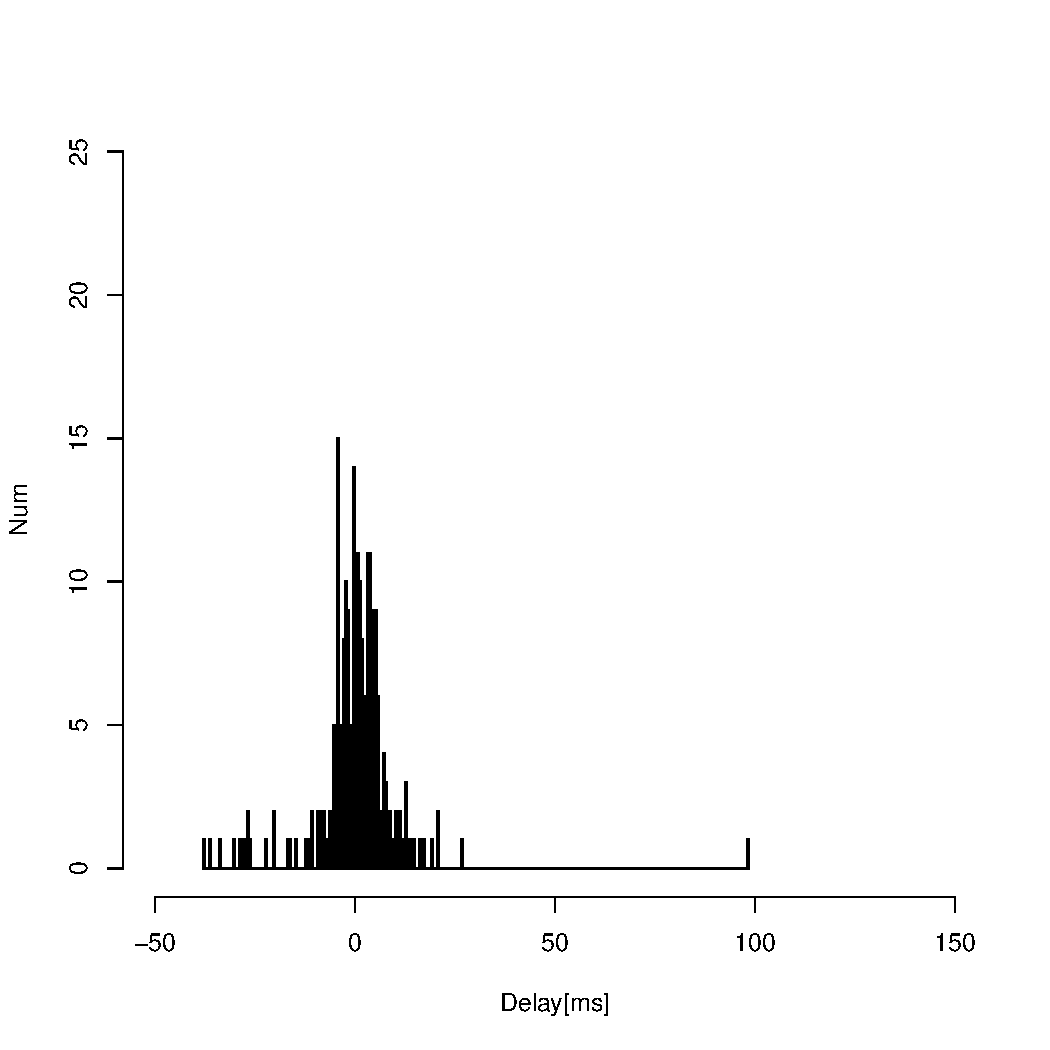
\includegraphics[width=.33\columnwidth]{C:/master/mstudy/paper/figure/0229_12-arma-normal-reshist.pdf}
}\\
\subfigure[17:00 - 18:00]{
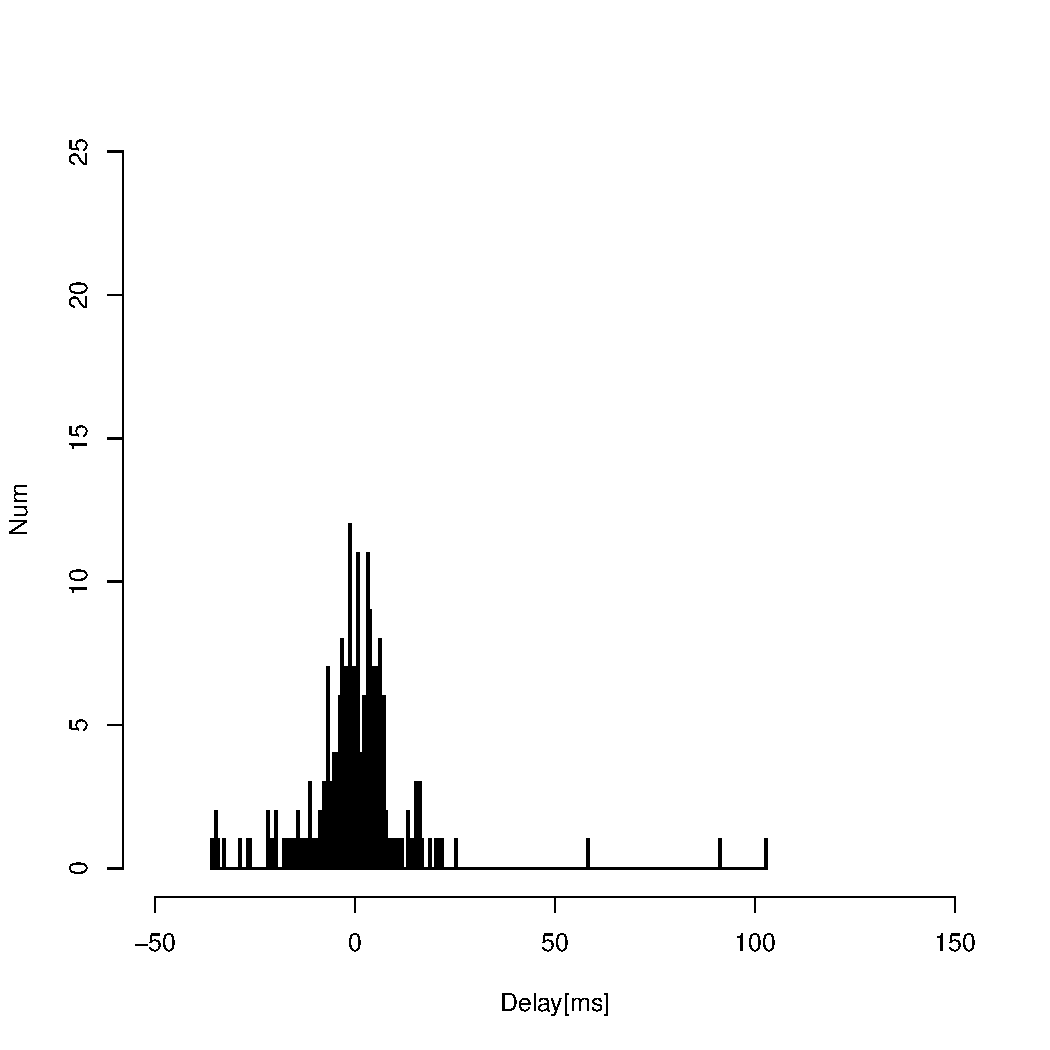
\includegraphics[width=.33\columnwidth]{C:/master/mstudy/paper/figure/0229_17-arma-normal-reshist.pdf}
}~
\subfigure[20:00 - 21:00]{
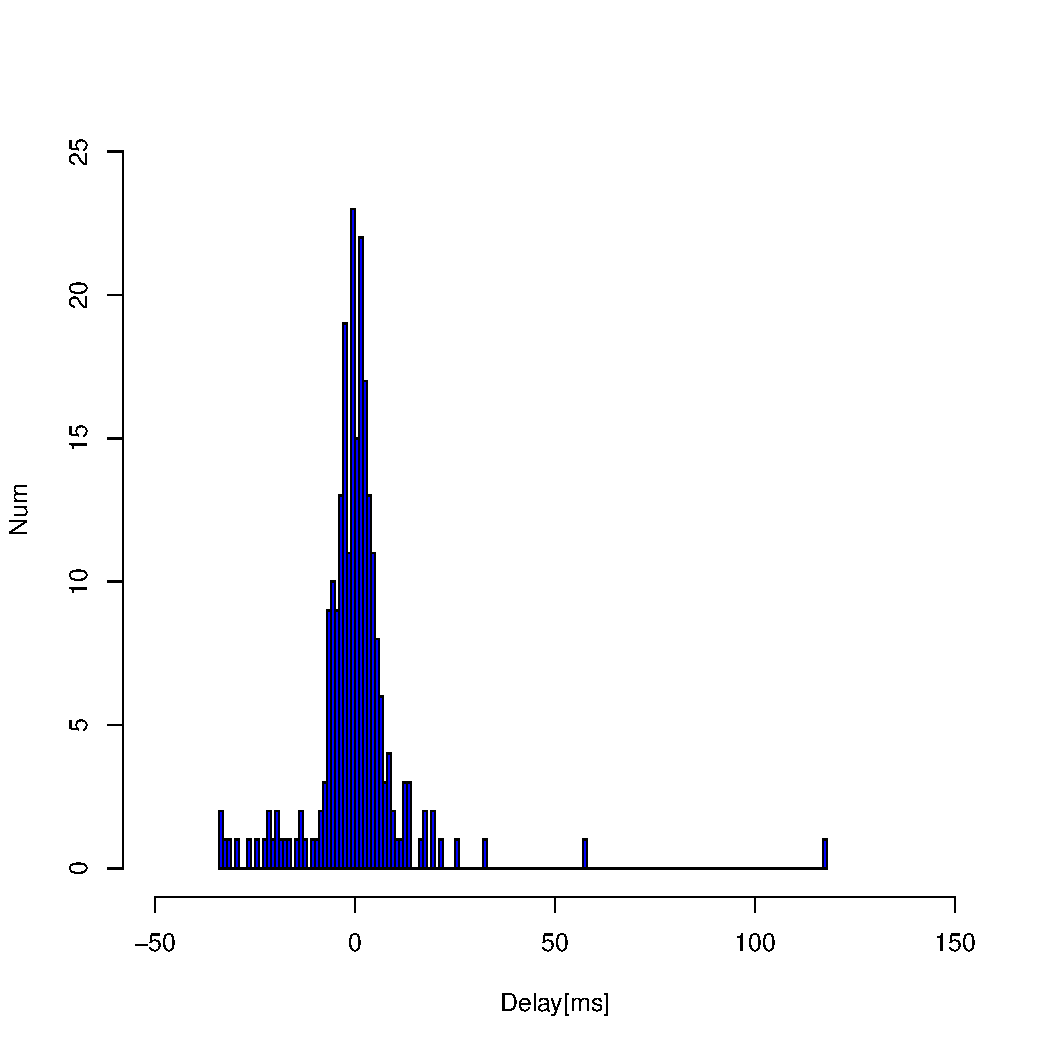
\includegraphics[width=.33\columnwidth]{C:/master/mstudy/paper/figure/0229_20-arma-normal-reshist.pdf}
}
\caption{図 \ref{reg1} の残差分布,ビン幅 1ms}
\label{res1}
\end{center}
\end{figure}

\begin{figure}[H]
\begin{center}
\subfigure[3:00 - 4:00]{
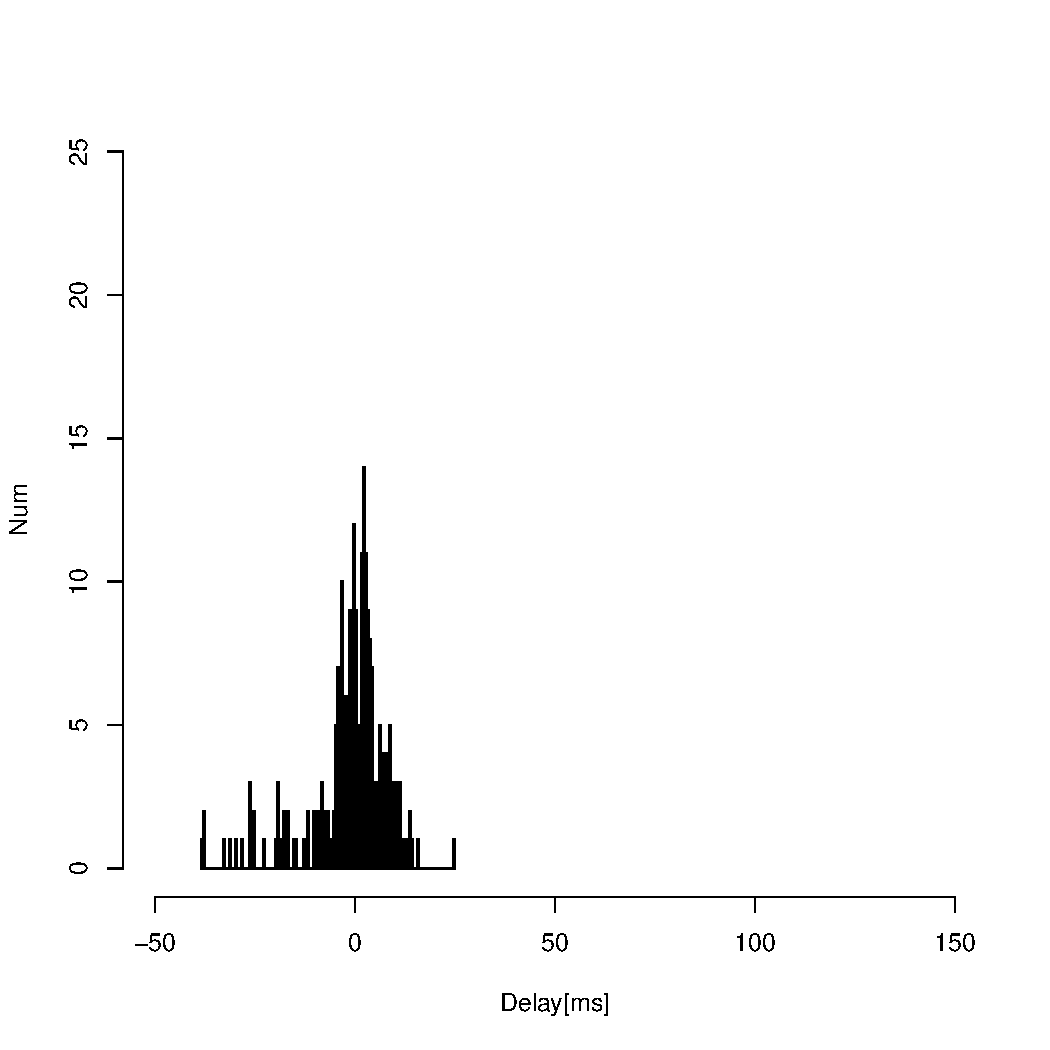
\includegraphics[width=.33\columnwidth]{C:/master/mstudy/paper/figure/0229_03-arma-diff-reshist.pdf}
}~
\subfigure[7:00 - 8:00]{
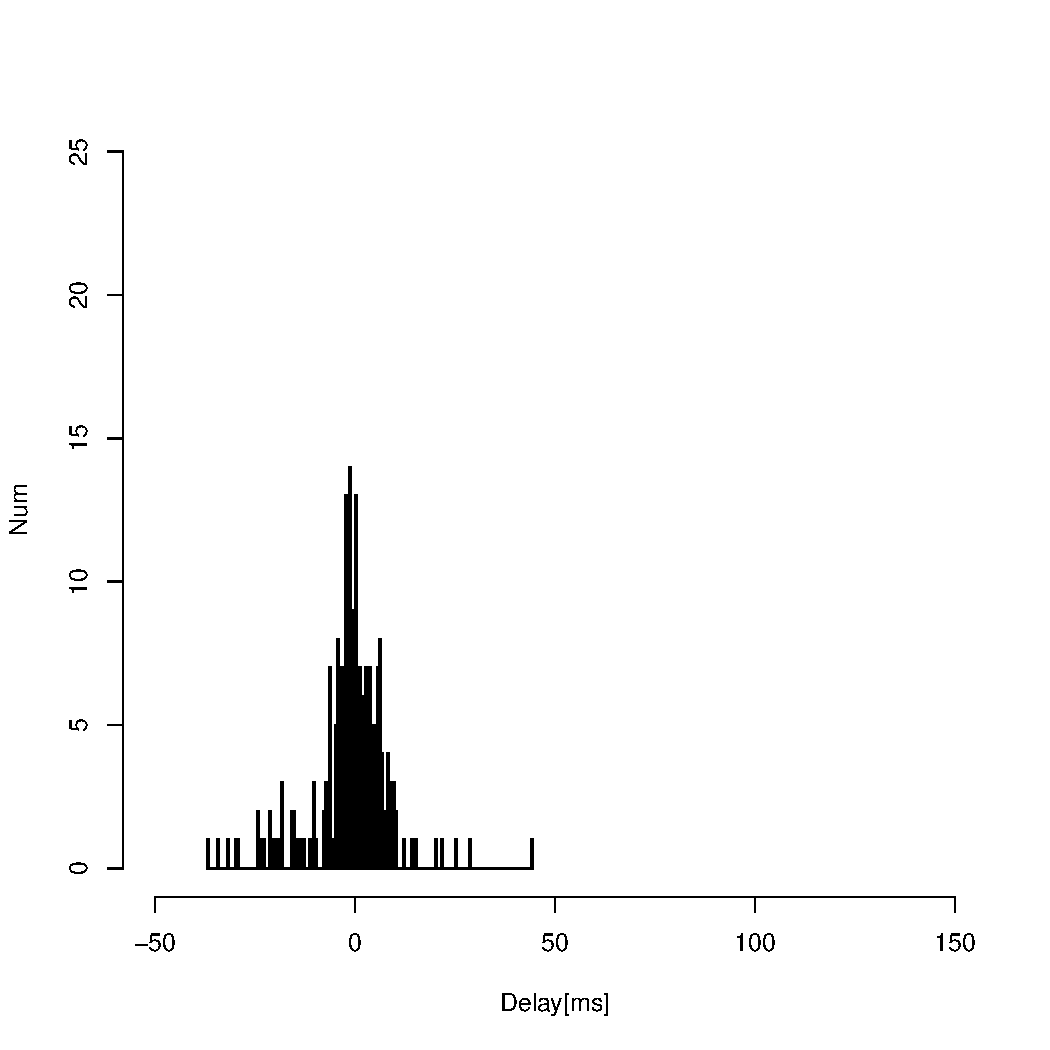
\includegraphics[width=.33\columnwidth]{C:/master/mstudy/paper/figure/0229_07-arma-diff-reshist.pdf}
}~
\subfigure[12:00 - 13:00]{
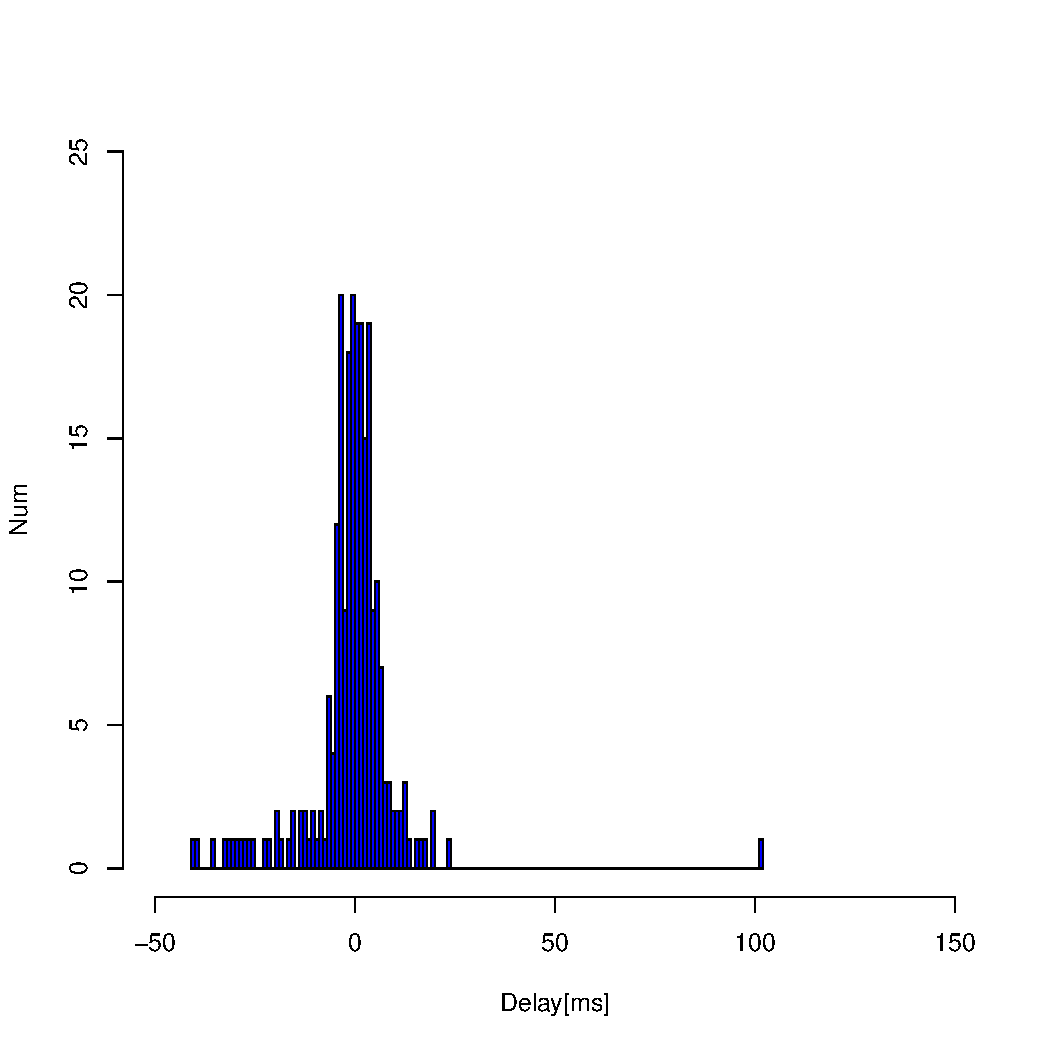
\includegraphics[width=.33\columnwidth]{C:/master/mstudy/paper/figure/0229_12-arma-diff-reshist.pdf}
}\\
\subfigure[17:00 - 18:00]{
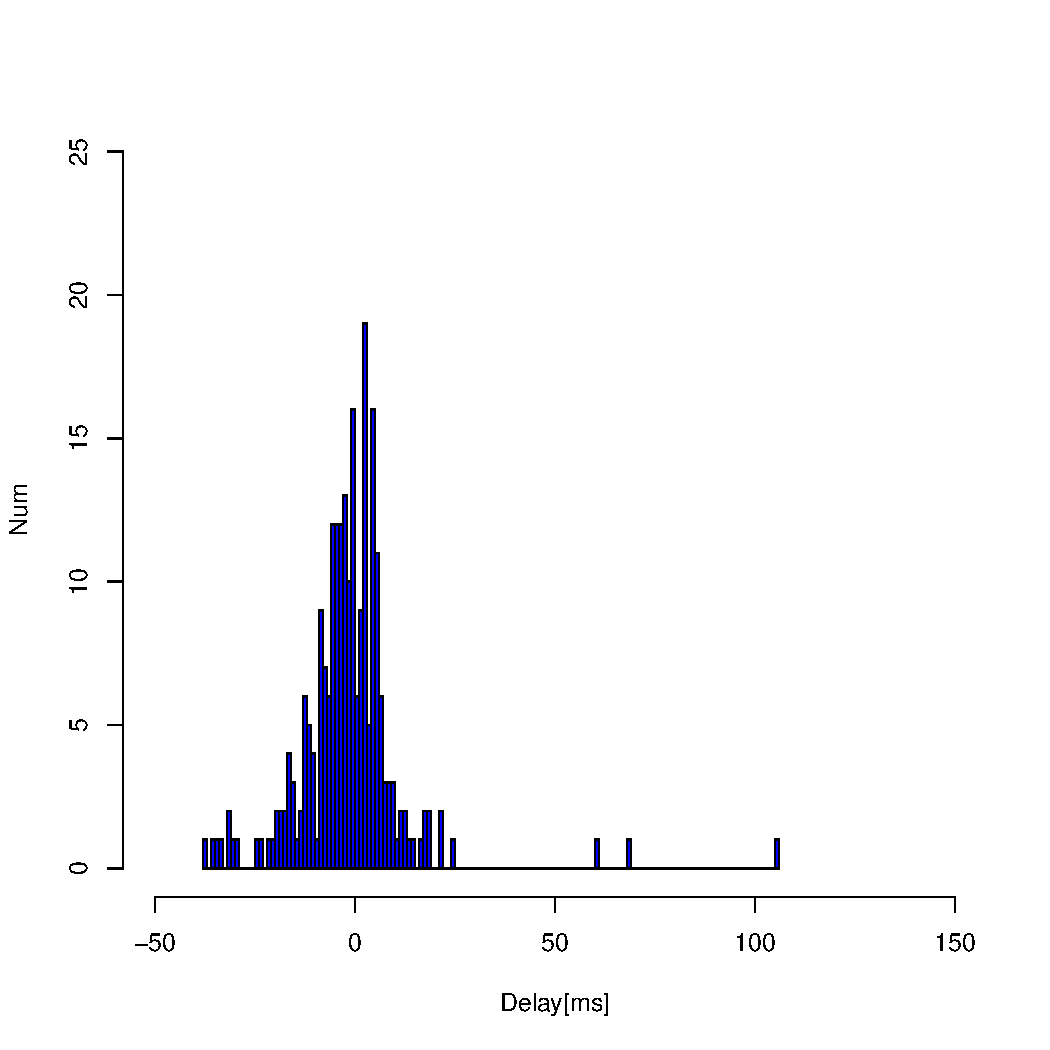
\includegraphics[width=.33\columnwidth]{C:/master/mstudy/paper/figure/0229_17-arma-diff-reshist.pdf}
}~
\subfigure[20:00 - 21:00]{
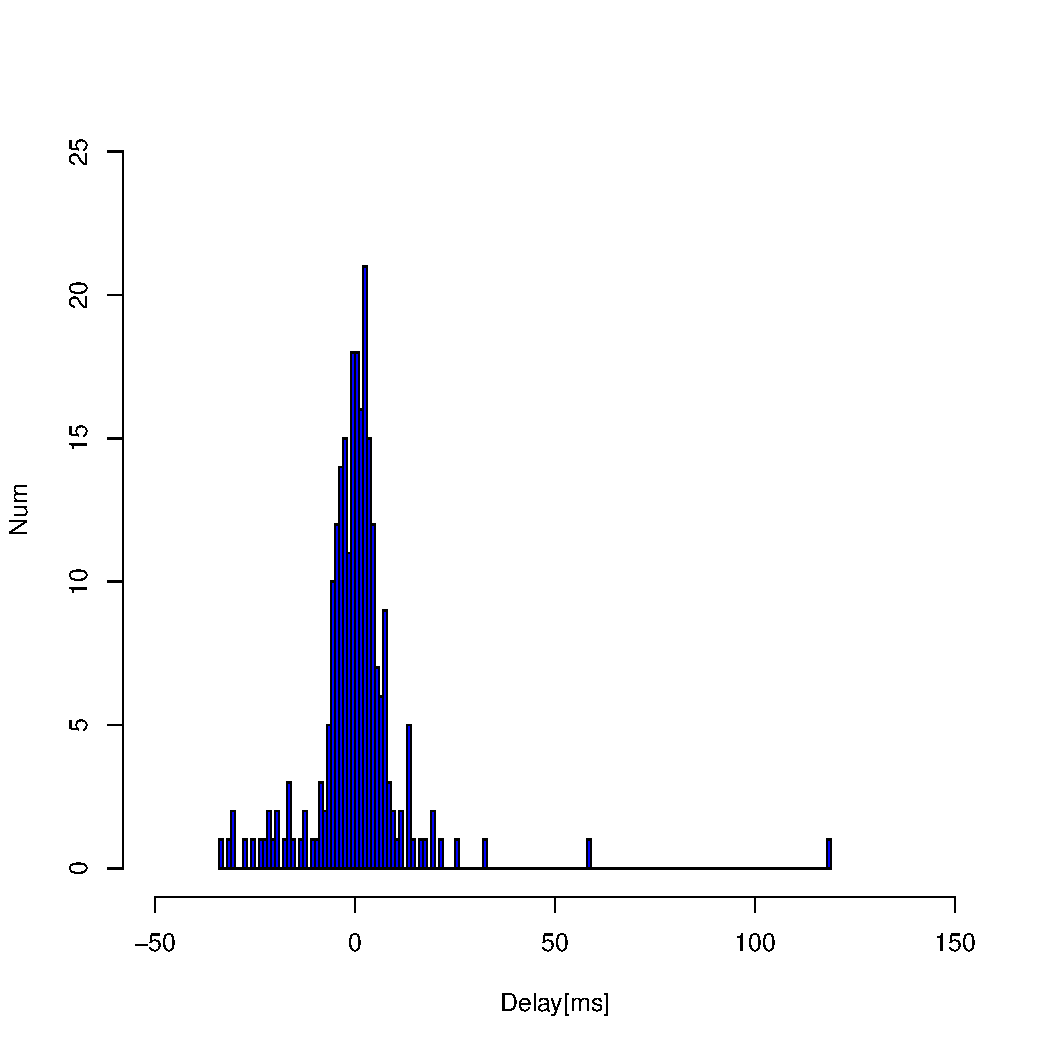
\includegraphics[width=.33\columnwidth]{C:/master/mstudy/paper/figure/0229_20-arma-diff-reshist.pdf}
}
\caption{図 4 の残差分布,ビン幅 1ms}
\end{center}
\end{figure}

\begin{figure}[H]
\begin{center}
\subfigure[3:00 - 4:00]{
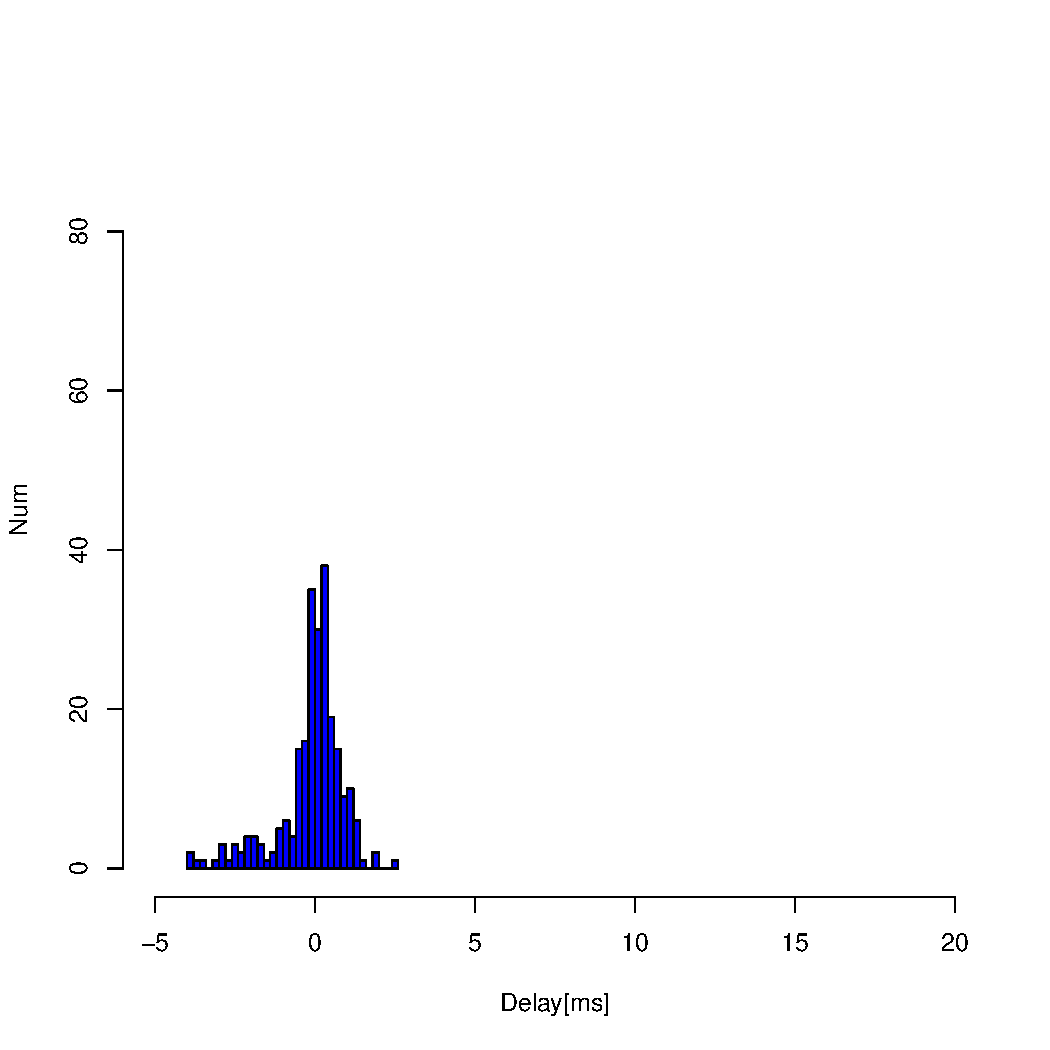
\includegraphics[width=.33\columnwidth]{C:/master/mstudy/paper/figure/0229_03-arma-ma-reshist.pdf}
}~
\subfigure[7:00 - 8:00]{
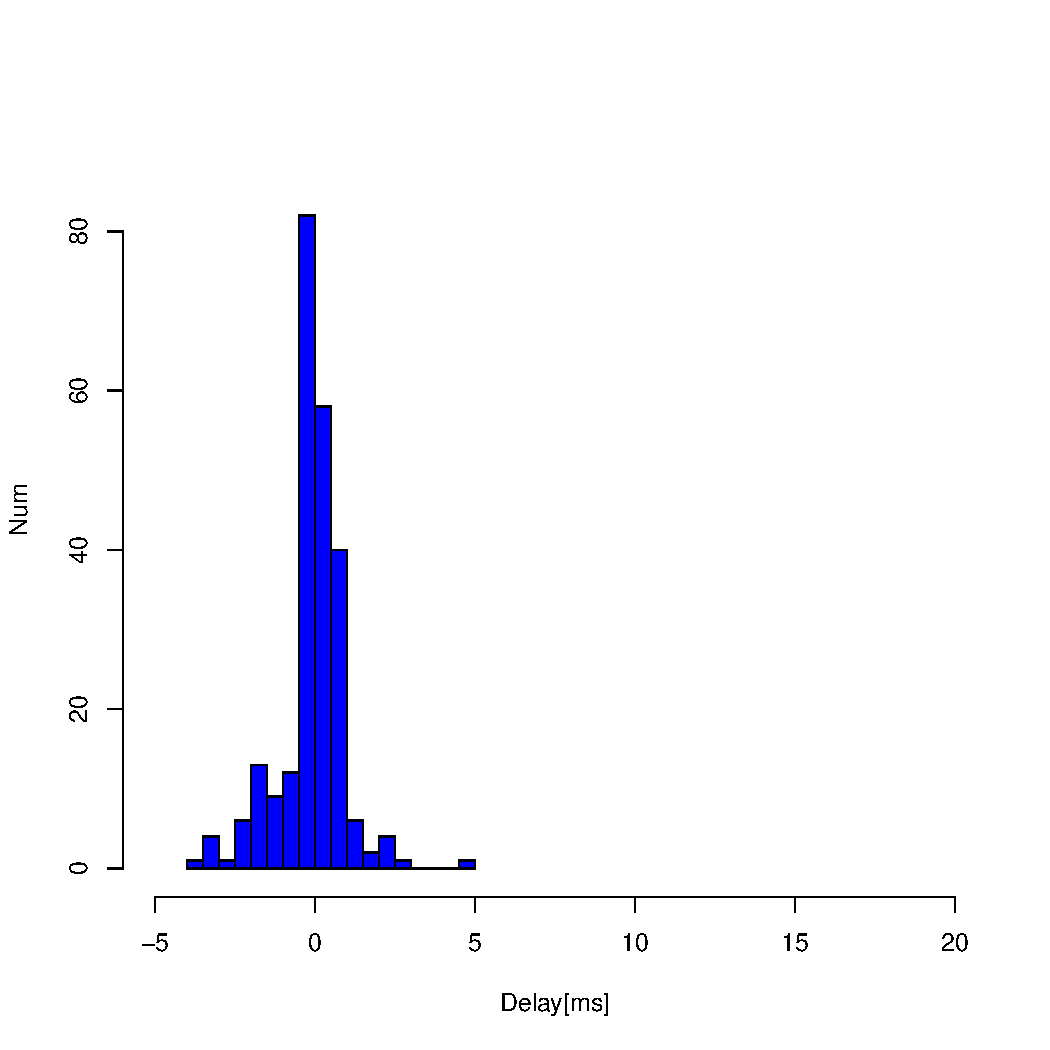
\includegraphics[width=.33\columnwidth]{C:/master/mstudy/paper/figure/0229_07-arma-ma-reshist.pdf}
}~
\subfigure[12:00 - 13:00]{
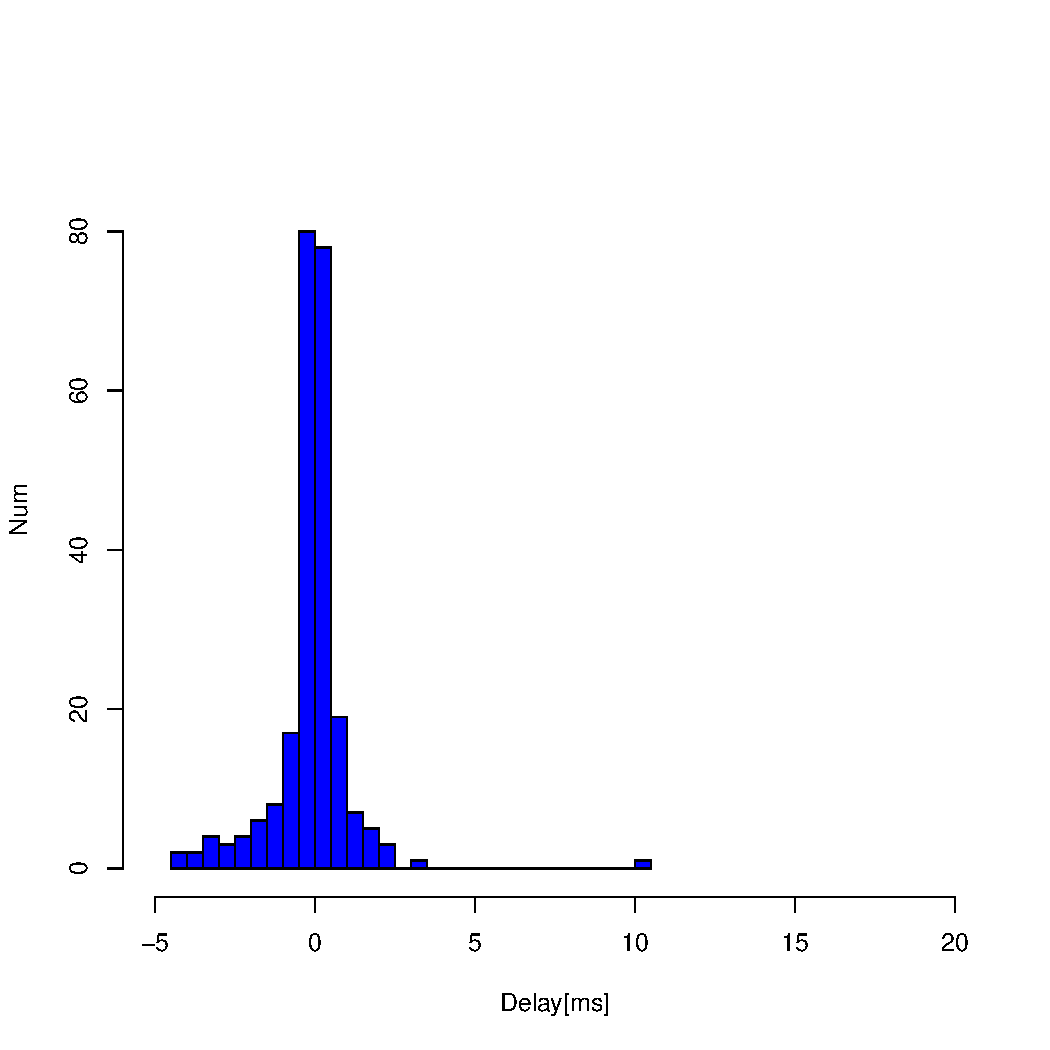
\includegraphics[width=.33\columnwidth]{C:/master/mstudy/paper/figure/0229_12-arma-ma-reshist.pdf}
}\\
\subfigure[17:00 - 18:00]{
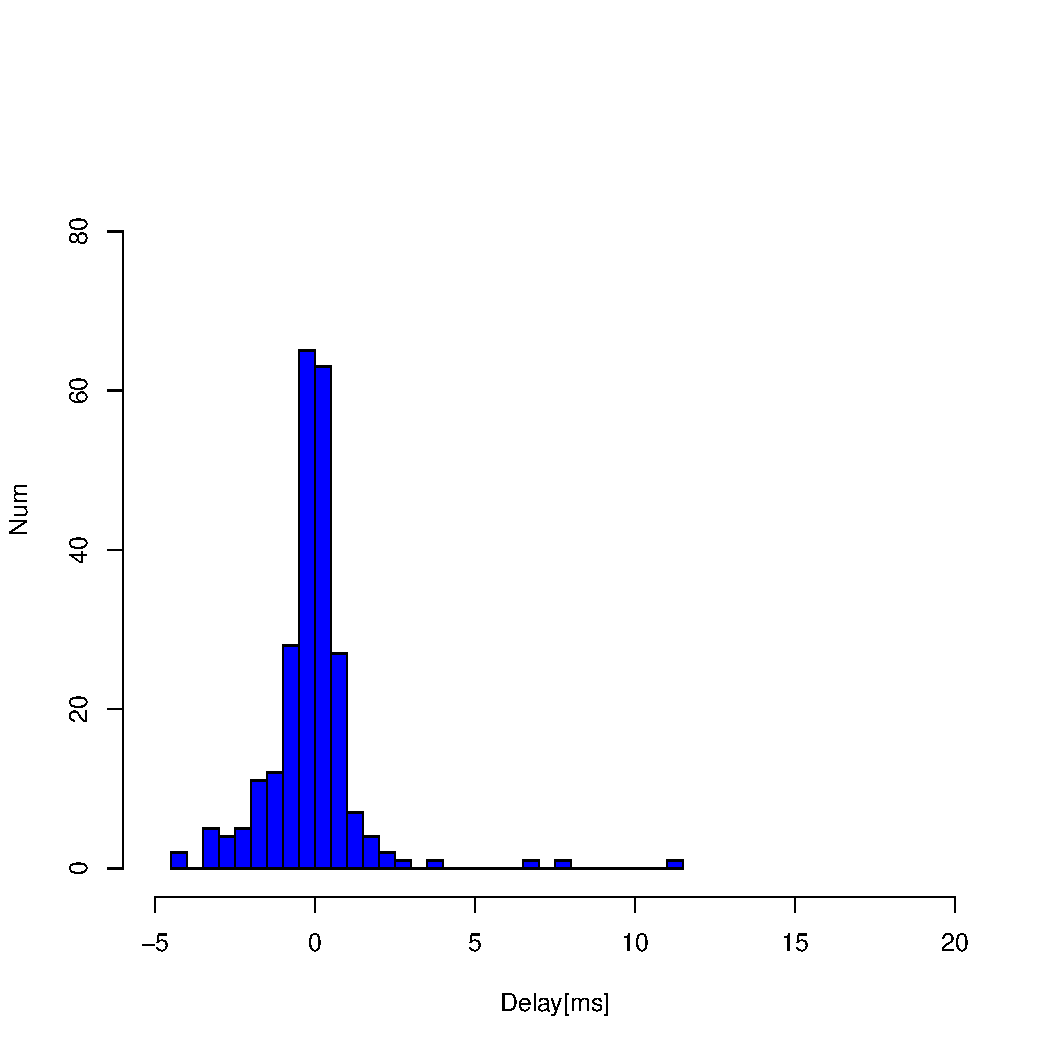
\includegraphics[width=.33\columnwidth]{C:/master/mstudy/paper/figure/0229_17-arma-ma-reshist.pdf}
}~
\subfigure[20:00 - 21:00]{
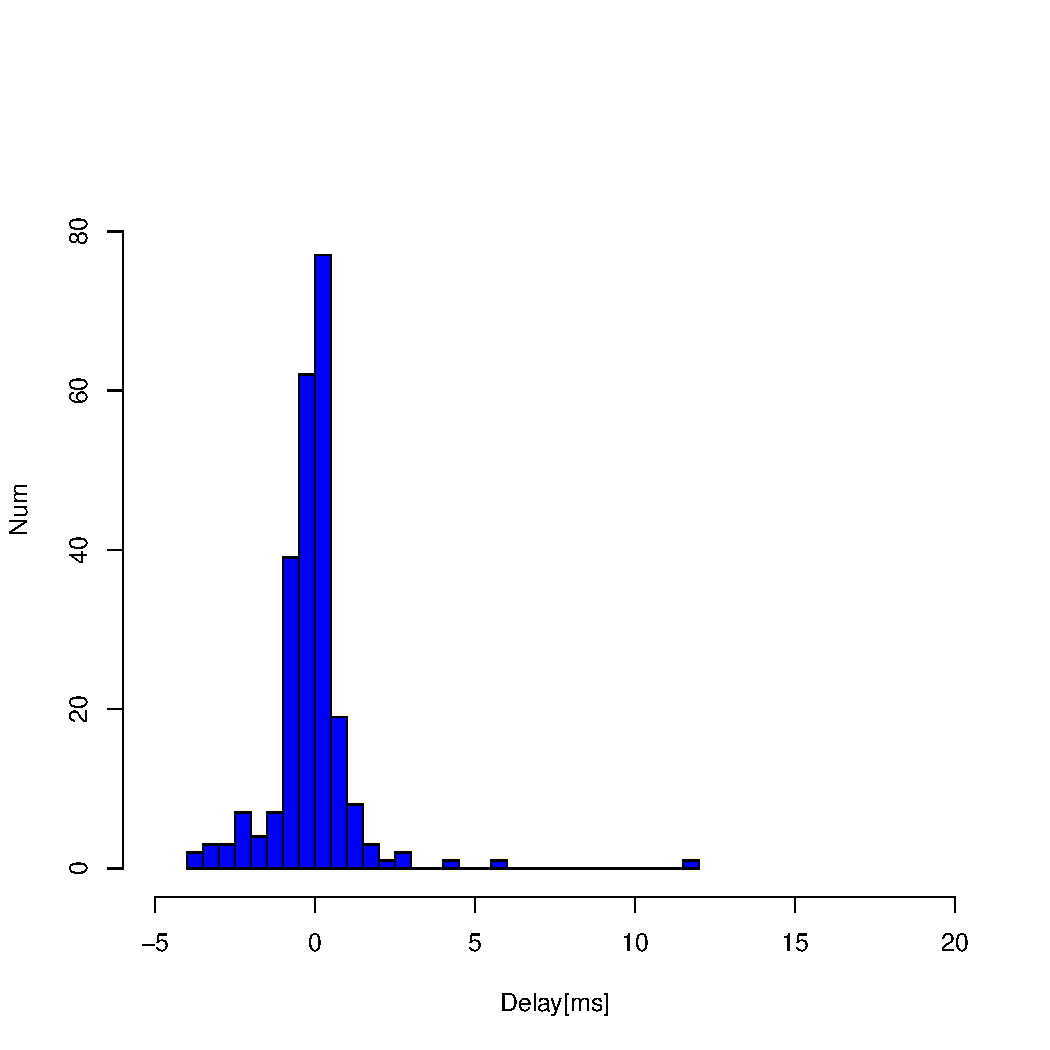
\includegraphics[width=.33\columnwidth]{C:/master/mstudy/paper/figure/0229_20-arma-ma-reshist.pdf}
}
\caption{図 \ref{reg2} の残差分布,ビン幅 1ms}
\label{res2}
\end{center}
\end{figure}

ここでは,残差の独立性を検証する手段の一つとして,リュング・ボックス検定を用いた.
これは,帰無仮説を検証データが互いに独立であるとし,対立仮説を検証データは互いに独立でないとした検定である.
また,残差の分布の正規性を検証する手段の一つとして,ジャック-ベラ検定を用いた.
これは,帰無仮説を検証データの分布が正規分布であるとし,対立仮説を検証データの分布が正規分布でないとした検定である.

2月29日(土) AWS サーバを対象とした ping 応答遅延に対する(i)(ii)(iii)での回帰結果において,それぞれの残差に対しリュング・ボックス検定とジャック-ベラ検定を用いたときのその p 値を表 \ref{t1} から表 \ref{t2} に示す.
\begin{table}[H]
\begin{center}
\caption{2月29日(土) AWS サーバを対象とした ping 応答遅延に対する(i)前処理なしでの ARMA モデル回帰における残差分析}
\label{t1}
\begin{tabular}{|c|l|l|}
\hline
 &リュング・ボックス検定の p 値&ジャック-ベラ検定の p 値\\
\hline
3:00-4:00&0.7299&2.2e-16 未満\\
\hline
7:00-8:00&0.9636&2.2e-16 未満\\
\hline
12:00-13:00&0.3704&2.2e-16 未満\\
\hline
17:00-18:00&0.9606&2.2e-16 未満\\
\hline
20:00-21:00&0.9649&2.2e-16 未満\\
\hline
\end{tabular}
\end{center}
\end{table}

\begin{table}[H]
\begin{center}
\caption{2月29日(土) AWS サーバを対象とした ping 応答遅延に対する(ii)差分処理での ARMA モデル回帰における残差分析}
\begin{tabular}{|c|l|l|}
\hline
 &リュング・ボックス検定の p 値&ジャック-ベラ検定の p 値\\
\hline
3:00-4:00&0.8654&2.2e-16 未満\\
\hline
7:00-8:00&0.8798&2.2e-16 未満\\
\hline
12:00-13:00&0.9473&2.2e-16 未満\\
\hline
17:00-18:00&0.9414&2.2e-16 未満\\
\hline
20:00-21:00&0.9691&2.2e-16 未満\\
\hline
\end{tabular}
\end{center}
\end{table}

\begin{table}[H]
\begin{center}
\caption{2月29日(土) AWS サーバを対象とした ping 応答遅延に対する(iii)移動平均での ARMA モデル回帰における残差分析}
\label{t2}
\begin{tabular}{|c|l|l|}
\hline
 &リュング・ボックス検定の p 値&ジャック-ベラ検定の p 値\\
\hline
3:00-4:00&0.6312&2.2e-16 未満\\
\hline
7:00-8:00&0.6252&2.2e-16 未満\\
\hline
12:00-13:00&0.5824&2.2e-16 未満\\
\hline
17:00-18:00&0.4843&2.2e-16 未満\\
\hline
20:00-21:00&0.3324&2.2e-16 未満\\
\hline
\end{tabular}
\end{center}
\end{table}

表 \ref{t1} から表 \ref{t2} において各時間帯のリュングボックス検定の p 値は全て有意水準 5\% としたときよりも大きな値をとっている.
そのため,(i)(ii)(iii)のそれぞれの回帰において,残差は互いに独立であるという帰無仮説は保留された.
しかし,ジャック-ベラ検定の p 値は有意水準 5\% としたときよりも小さい値をとっており,(i)(ii)(iii)のそれぞれの回帰において,残差の分布は正規分布に従っていないという結果となった.

これは,計測データにおいて単発的な大きなもしくは小さな値の応答遅延が存在し,過去直近の計測データから回帰を行う ARMA モデルではこれらの単発的な応答遅延に対する残差の絶対値が大きくなる.
さらに,これらの単発的な応答遅延の発生頻度が少なくないことから,残差分布の裾部分が正規分布から外れることが原因と考えられる.

\section{今後の予定}
\begin{itemize}
\item 原稿を執筆します
\item ARMA-GARCHモデルを用いて同様の検証を行います.
\end{itemize}
\section{原稿章構成}
\begin{table}[H]
\begin{tabular}{ll}
1&はじめに\\
2& LTE の概要\\
3&計測実験の設定\\
4&時系列モデリングによる分析\\
&要検討\\
&4.1 時系列モデリングにおける次数の設定\\
&4.2 ARIMA モデルによる回帰\\
&4.3 ARMA-GARCH モデルによる回帰\\
5&クラスタリングによる分類\\
6&まとめ
\end{tabular}
\end{table}
\section{スケジュール}
\begin{table}[H]
\begin{tabular}{|c|c|}
\hline
日付&予定\\
\hline
3/26&この日の週報から原稿の途中経過を報告させていただきます\\
\hline
4月中旬&原稿締め切り\\
\hline
5/21 - 5/22&IN研究会\\
\hline
\end{tabular}
\end{table}
原稿執筆後 : 抄録とキーワードの登録(日本語と英語)

プログラム決定後 : 参加費支払い

5/14~ : 技報ダウンロード開始

\bibliography{reference}
\bibliographystyle{ieeetr}
\end{document}